\chapter{Quantum Algorithms}
\lecture{9}{7 Oct. 10:30}{}
\section{Introduction}
이번 챕터에서 우리는 \textit{Quantum Algorithm}에 대해 다루고자한다. Quantum algorithm은 quantum circuit이나 quantum computer에서 구현되는 알고리즘을 지칭한다.
Classical computer가 어려운 문제를 해결하기 위하여 만들어진 것처럼, quantum algorithm에 대해서 공부하고 새로운 방식을 고안하는 것은 quantum computer의 동작방식과 quantum computer의 한계를 분석하기 위한 중요한 과제이다. 
Quantum computer라는 개념이 등장하고 나서부터 지금까지 많은 종류의 quantum algorithm들이 고안되어 왔다. 이번 강의에서 다루고자하는 quantum algorithm은 다음과 같다. 
\begin{itemize}
  \item Elementary quantum algorithms
  \item Hamiltonian simulations
  \item Quantum Fourier transform
  \item Phase estimation
  \item Quantum search algorithm (Grover search algorithm)
  \item Amplitude amplification / estimation algorithms
  \item HHL algorithm
\end{itemize}

\section{Elementary quantum algorithms using quantum parallelism}

Quantum mechanics만의 특징을 이용할 수 있는 quantum computer는 \textit{Quantum parallelism}이라는 특성을 가진다. 이는 quantum computer가 특정 oracle; function $f(x)$에 대하여 동시에 여러개의 입력에 대한 결과를 병렬적으로 얻을 수 있다는 의미이다.
고전적인 개념인 $f(x)$를 quantum computer에서 실행하기 위해서는, quantum computer의 연산단위인 \textit{unitary operator}로 함수를 표현해야하는 필요가 있다.

먼저, 간단한 one-bit boolean function $f : \{0, 1\} \rightarrow \{0, 1\}$를 생각해보자.
직관적으로, 이 함수에 대응되는 operator는 다음과 같이 설계할 수 있다. 이 operator는 $f(0) = 1$이라면, $U_f\ket{0} = \ket{1}$처럼 동작하도록 quantum gate들을 이용하여 구현된다.
\begin{equation*}
  \ket{x} \xrightarrow{U_f} \ket{f(x)}
\end{equation*}
그러나 이러한 방식으로 operator를 설계하게 되면, \textit{non-invertible} 함수 $f(x)$에 대한 operator는 더이상 unitary 조건을 만족하지 못한다.
따라서 이 문제를 해결하기 위하여 control을 수행하는 추가적인 input qubit을 추가하여 unitary operator가 되도록 설계한다.
\begin{definition}[Unitary oracle]\label{def:oracle-gate}
    함수 $f$에 대한 unitary operator $U_f$는 다음과 같이 정의된다.
    \begin{equation*}
      \ket{x}\ket{y} \xrightarrow{U_f} \ket{x}\ket{y \oplus f(x)}
    \end{equation*}
\end{definition}

\newpage 

$\ket x$는 $f$의 입력으로 사용되는 \textbf{oracle qubit}이며, $\ket y$는 1일때는 $f(x)$의 결과를 flip 시키고 0일 때는 $f(x)$의 결과를 반환하는 역할을 수행한다.
그럼 이렇게 설계한 unitary operator에 \textit{superposition state}를 $\ket x$로 제공하면 결과적으로 우리는 다음과 같은 two-qubit state를 얻게 된다.
\begin{equation*}
  \ket{+}\ket{y} \xrightarrow{U_f} \frac{1}{\sqrt 2} (\ket{0}\ket{f(0)} + \ket{1} \ket{f(1)})
\end{equation*}

즉, one-bit boolean function에서 가능한 모든 입력 0, 1에 대한 출력을 $U_f$를 한 번 호출함으로써 얻게 된 것이다!
Classical computer에서 병렬연산은 서로 다른 컴퓨팅 자원을 사용할 뿐, $f$를 여러번 호출해야하는 사실은 변하지 않지만, quantum computer에서의 병렬연산은 실제로 $f$를 한 번 호출하여 모든 연산을 수행할 수 있다.

이렇게 어떤 함수 $f$에 대응되는 unitary operator를 설계하는 것은 n-bit boolean function에 대해서 쉽게 일반화할 수 있다.
$n$-bit boolean function $f: \{0, 1\}^n \rightarrow \{0, 1\}$에 대응되는 unitary operator는 Definition~\ref{def:oracle-gate}을 이용하여 쉽게 설계할 수 있으며, 더 나아가 $n$-qubit에 대한 superposition state를 입력으로 제공하면 다음 결과를 얻게된다.
\begin{equation*}
  \frac{1}{\sqrt{2^n}} \sum_{x \in\{0,1\}^n}|x\rangle|0\rangle \rightarrow \frac{1}{\sqrt{2^n}} \sum_{x \in\{0,1\}^n}|x\rangle|f(x)\rangle
\end{equation*}
이 회로를 이용하면 한 번의 연산만으로 $2^n$개의 입력에 대한 출력을 동시에 얻을 수 있다.
그러나 한 가지 주의해야할 점은, 우리가 결과를 측정하는 순간 여러개의 superposition output은 사라지고 확률에 따라서 단 하나의 결과만을 얻을 수 있다는 사실이다. 
따라서 이러한 quantum parallelism만의 독특한 특징을 잘 활용하여 효과적인 연산을 수행할 수 있도록 알고리즘을 설계하는 것이 중요하다.

이 강의에서는 parallelism의 장점을 활용하는 대표적인 알고리즘들(e.g., Deutsch’s algorithm, Deutsch-Josza algorithm, Simon’s algorithm, and Bernstein-Vazirani algorithm)에 대해 소개한다.

\subsection{Deutsch’s algorithm}
Deutsch’s algorithm은 주어진 one-bit boolean function $f$이 \textbf{balance}인지 \textbf{constant}인지를 판단하는 문제를 해결한다.\footnote{constant: $f(0)=f(1)$, balance: $f(0)\ne f(1)$}
Classical computer가 이 문제를 해결하기 위해서는 두 함숫값 $f(0), f(1)$을 비교하기 위해서 반드시 2번의 함수 호출이 필요하다.
그러나, 지금부터 우리는 quantum computer는 \textbf{단 한번}의 gate call만으로 이 문제를 해결할 수 있음을 보이고자한다.

\begin{enumerate}
  \item input state
  : 우리는 다음과 같은 state를 input으로 제공한다.
  \begin{equation*}
    \ket{\psi} = \ket 0 \ket 1
  \end{equation*}
  \item apply Hadamard gates on both qubits
  : $H$ gate를 가하면, 다음과 같은 상태로 변화한다.
  \begin{equation*}
    \ket{\psi} = \ket + \ket -
  \end{equation*}
  \item apply $U_f$
  : operator를 통과한 state는 다음과 같다.\footnote{$\ket{f(x)} - \ket{1 \oplus f(x)}$는 $f(x)$의 값에 따라서, $\ket{0} - \ket{1}$ ($f(x) = 0$) 또는 $\ket{1} - \ket{0}$ ($f(x) = 1$)이 된다.}
  \begin{align*}
    \ket{\psi} &= U_f\left(\frac{1}{2}\left(\ket{00} + \ket{10} - \ket{01} - \ket{11} \right)\right)\\
                &= \frac{1}{2}\left(\ket{0, f(0)} \ket{1, f(1)} - \ket{0, 1 \oplus f(0)} - \ket{1, 1 \oplus f(1)}\right)\\
                &= \frac{1}{2}\Big(\ket{0}(-1)^{f(0)}(\ket 0 - \ket 1) + \ket{1}(-1)^{f(1)}(\ket 0 - \ket 1) \Big) \\
                &= \frac{1}{2} \sum_{x \in \{0, 1\}}(-1)^{f(x)} \ket x (\ket 0 - \ket 1)
  \end{align*}
  따라서 각 case에 대해 state는 다음의 2가지 모습을 띄게 된다.
  \begin{equation*}
  \ket{\psi} = \begin{cases}
    \pm \ket + \ket - & \text{ if } f(0) = f(1)\\ 
    \pm \ket - \ket - & \text{ if } f(0) \ne f(1)
  \end{cases}
  \end{equation*}
  \item apply again Hadamard gates on oracle qubit
  : 마지막으로 oracle qubit에 $H$ gate를 가하면, $f$의 종류에 따라서 다음과 같은 상태가 된다.
  \begin{equation*}
    \ket{\psi} = \begin{cases}
      \pm \ket 0 \ket - & \text{ if } f(0) = f(1)\\ 
      \pm \ket 1 \ket - & \text{ if } f(0) \ne f(1)
    \end{cases}
  \end{equation*}
\end{enumerate}

따라서, oracle qubit을 측정하면, 100\%의 확률로 0 또는 1의 값을 얻게될 것이며, 그 값에 따라서 우리는 $f$가 balance인지 constant인지를 다음 규칙에 따라서 쉽게 판단할 수 있다. $\Box$
\begin{equation*}
  \ket{\psi} = \begin{cases}
    constant & \text{ if } q_o = 0\\ 
    balance & \text{ if } q_o = 1
  \end{cases}
\end{equation*}

Deutsch’s algorithm은 classical algorithm보다 quantum algorithm 알고리즘이 더 효과적임을 보인 첫 번째 알고리즘이다. 하지만, 그 효과는 단지 2번의 호출을 1번으로 줄일 뿐이다.
따라서 지금부터 더 효과적인 알고리즘들에 대해서 소개하고자한다.

\lecture{10}{14 Oct. 10:30}{}
\subsection{Deutsch-Jozsa algorithm}
Deutsch-Jozsa algorithm은 간단히 말하자면, one-bit boolean function에 대한 문제인 Deutsch-Jozsa algorithm을 $n$-bit boolean function에 대한 문제로 일반화한 것이다.
즉, $n$-bit boolean function $f: \{0, 1\}^n \rightarrow \{0, 1\}$이 \textbf{constant}인지 \textbf{balanced}인지를 판단하는 문제를 해결하는 알고리즘이다.\footnote{여기서 말하는 balanced는 $2^n$개의 input중에서 $2^{n-1}$개의 input에 대한 결과가 0이고, 나머지 $2^{n-1}$개의 input에 대한 결과가 1인 경우를 의미한다.}
마찬가지로 classical computer가 이 문제를 해결하기 위해서는 최대 $2^{n-1}+1$개의 function value를 비교해야하기 때문에 $2^{n-1}+1$번의 함수 호출을 필요로한다. 그러나, 지금부터 이런문제를 해결하려고 할 때도, quantum computer는 \textbf{단 한번}의 gate call만으로 이 문제를 해결할 수 있음을 보일 것이다.

\begin{enumerate}
  \item input state
  : 우리는 다음과 같은 state를 input으로 제공한다. $\{0, 1\}^n$의 가능한 모든 input을 나타내기 위하여, oracle qubit은 $n$개의 qubit으로 구성된다.
  \begin{equation*}
    \ket{\psi} = \ket{0}^{\otimes n} \ket 1
  \end{equation*}
  \item apply Hadamard gates on both qubits: 이때, $\ket{+}^{\otimes n}$은 가능한 모든 $2^n$개의 $n$-bit string들의 superposition이기 때문에, 다음과 같이 표현할 수 있다.
  \begin{align*}
    \ket{\psi} &= \ket{+}^{\otimes n} \ket - \\
              &= \sum_{x \in \{0, 1\}^n} \frac{1}{\sqrt{2^{n}}} \ket x  \frac{1}{\sqrt 2}(\ket 0 - \ket 1)
  \end{align*}
  \item apply $U_f$
  : operator를 통과한 state는 다음과 같다. (Deutsch’s algorithm의 표현을 이용하자)
  \begin{align*}
    \ket{\psi} &= U_f  \frac{1}{\sqrt{2^{n+1}}} \Big(\sum_{x \in \{0, 1\}^n} \ket x  (\ket 0 - \ket 1)\Big)\\
              &= \frac{1}{\sqrt{2^{n+1}}} \sum_{x \in \{0, 1\}^n} (-1)^{f(x)} \ket x  (\ket 0 - \ket 1)
  \end{align*}
  \item apply again Hadamard gates on oracle qubit
  : $H$ gate를 임의의 $n$-qubit computational basis에 가한 결과는 다음과 같다. 이는 single qubit에 대한 동작을 $n$-qubit에 대해 \textit{독립적으로} 적용한 결과이다.
  \begin{equation}
    H^{\otimes n} \ket x = \frac{1}{\sqrt{2^n}} \sum_{z \in \{0, 1\}^n} (-1)^{x \cdot z} \ket z 
  \end{equation}\label{eq:tensor-H}
  이를 이용하여 $H$ gate를 적용한 state를 표현하면, 다음과 같다.
  \begin{equation*}
    \ket \psi  = \frac{1}{{2^n}} \sum_{x, z \in \{0, 1\}^n} (-1)^{f(x) + x \cdot z} \ket z \ket{-}
  \end{equation*}
  
  만약 $f(x)$가 constant function이라면, $\forall x$에 대해서 $f(x)$의 값은 항상 동일하기 떄문에, $(-1)^{f(x)}$의 값이 $+1$, 또는 $-1$이라는 constant가 되어 다음과 같이 나타낼 수 있다.
  \begin{align*}
  \left|\psi\right\rangle= \pm \frac{1}{{2^{n}}} \sum_{x, z \in\{0,1\}^n} {(-1)^{x\cdot z}|z\rangle} \ket -
  \end{align*}
  $z = 0^n$인 경우를 가정해보자. 이는 $x$가 어떤 값이 되던지간에 $x\cdot z$ \footnote{ $x \cdot z = x_1 z_1 + x_2 z_2 + \cdots + x_n z_n \mod 2$ }의 값이 0이 되기 떄문에, 다음과 같이 표현할 수 있게 된다.
  $\ket{0}^{\otimes n}$의 amplitude의 square norm이 1이기 때문에, 100\% 확률로 $0^n$을 측정할 수 있다.
  \begin{align*}
    \pm \frac{1}{{2^n}} \sum_{x \in\{0,1\}^n} (-1)^{x\cdot 0^n} |0\rangle^{\otimes n} \ket - = \pm \frac{1}{{2^n}}{2^n} \ket{0}^{\otimes n} \ket - = \boxed{\pm \ket{0}^{\otimes n} \ket -} 
  \end{align*}
  반면, $f(x)$가 balance function이라면, $f(x)$의 값이 $0$인 경우와 $1$인 경우가 정확히 1/2씩 나타나기 때문에, 각 항들이 소거되면서 $z=0^n$에 대한 amplitude가 0이 된다.
  \begin{align*}
    \Big(\frac{1}{{2^n}} 2^{n-1} |0\rangle^{\otimes n} \ket - \Big) + \Big( - \frac{1}{{2^n}} 2^{n-1} |0\rangle^{\otimes n} \ket - \Big) = \boxed{0 \ket{0}^{\otimes n} \ket -} 
  \end{align*}
\end{enumerate}
따라서, oracle qubit을 측정한 결과가 $0^n$인지 확인하여, $f$가 constant인지 balanced인지를 알 수 있다. $\Box$
  \begin{equation*}
    \ket{\psi} = \begin{cases}
      constant & \text{ if } q_o = 0^n\\ 
      balance & \text{ if } q_o \ne 0^n
    \end{cases}
  \end{equation*}

\section{Hamiltonian simulations}
Hamiltonian simulation은 quantum computer가 고안된 핵심적인 이유 중 하나이다. 리처드 파인만의 말을 인용하자면 자연, 그중에서도 특히 미시세계는 고전역학을 따르지 않기때문에, quantum mechanical을 따르는 simulation이 필요하다.
\begin{note}
  \textit{Nature isn’t classical, dammit, and if you want to make a simulation of nature, you’d better make it quantum mechanical, and by golly it’s a wonderful problem, because it doesn’t look so easy.}
\end{note}

Hamiltonian simulation은 간단히 말해 quantum state의 time evolution을 구하는 것이다. Schrödinger equation에 의하면, initial state $\ket{\psi(0)}$의 시간 $t$에 대한 time evolution은 다음과 같이 주어진다.
\begin{equation*}
  |\psi(t)\rangle=e^{-i H t}|\psi(0)\rangle
\end{equation*}

이 방정식을 곧바로 해결하여 문제를 풀 수도 있지만, Hamiltonian matrix의 크기가 exponential하게 증가하기 때문에 이를 classical algorithm으로 효과적으로 해결하기는 어렵다.

\subsection{Solution of Hamiltonian simulations}
우리는 \hyperref[def:k-local-Hamiltonian]{k-local Hamiltonian}을 이용하여 Hamiltonian simulation 문제를 해결하고자 한다.
\begin{definition}\label{def:k-local-Hamiltonian}
  $k$-local\footnote{여기서 local은 geometrically local이 아니라 단순히 system의 '개수'를 나타내기 위해 사용된다.} Hamiltonian은 주어진 $H$가 $n$-qubit system에서 \textbf{최대 $k$개의 system}에 대해서만 동작하는 $H_i$들의 합으로 표현되는 Hamiltonian이다. (이때 $L$은 $n$에 대해 polynomial이다.)
  $$ H=\sum_{i=1}^L H_i $$
\end{definition}

\begin{eg}
  예를 들어, 다음과 같이 정의되는 Hamiltonian은 2개의 system (2, 4)에 대해서만 동작한다.
  $$ H_i = I_1 \otimes Z_2 \otimes I_3 \otimes X_4 \otimes I_{\perp} $$
\end{eg}

\newpage 
Hamiltonian이 k-local Hamiltonian이라고 가정할 때, 이를 이용하여 어떻게 문제를 해결할 수 있을까?
그 아이디어는 단순하다. $e^{-i H t}$를 계산하는 것은 어렵지만, $e^{-i H_i t}$는 최대 $k << n$ subsystem에만 작용하기에 더 단순하며, 그 단순성 덕분에 quantum circuit을 사용하여 시뮬레이션 하기 쉽다.

만약, $[H_j, H_k] = 0$\footnote{$[H_j, H_k] = H_jH_k - H_kH_j$}이 성립한다면 $e^{-iHt} =e^{-i \sum H_j t} = \prod e^{-i H_j t}$\footnote{지수함수의 성질이 성립하기 위해서 필요한 조건. 실수들은 항상 commutative하기 때문에 이 성질이 자명하게 정립되었던 것}가 성립하기 때문에, 각각의 $H_i$에 대한 time evolution을 독립적으로 계산한 결과를 곱하여 전체 time evolution을 쉽게 구할 수 있다.
그러나 일반적으로 $[H_j, H_k] = 0$은 성립하지 않기 떄문에, 우리는 \hyperref[thm:trotter-formula]{Trotter formula}를 이용한다.

\begin{theorem}[Trotter formula]\label{thm:trotter-formula}
  Hermitian operator $H_j, H_k$에 대하여, 어떤 $t$에 대해서도 다음이 성립한다.\footnote{직관적으로, 주어진 time $t$ 대신에, 매우 짧은 시간간격인 $t/m$에 대한 time evolution을 $m$번 반복하여 $t$에 대한 time evolution을 근사할 수 있다는 것을 의미한다.}
  $$ e^{i (H_j + H_k) t} = \lim_{m \to \infty} \left( e^{i H_j t/m} e^{i H_k t/m} \right)^m $$ 
  이는 $H_j, H_k$가 not-commute라 하더라도 항상 성립한다.
\end{theorem}

\vspace{1em} 

따라서 $L=2$인 k-local Hamiltonian $H = H_1 + H_2$에 대해, Hamiltonian simulation을 수행하는 propagator $\tilde U (t) = e^{-i H_1t} e^{-i H_2 t}$를 시간에 대해서 미분하면, 다음과 같이 전개할 수 있다.
(with initial condition $\tilde U(0) = I$)
\begin{itemize}
  \item Eq.~\eqref{eq:expand-2}: $H_1, H_2$는 matrix라서 순서를 바꿀 수 없기에, 다른 항을 더하여 항을 정리하고 다시 뺀다.
  \item Eq.~\eqref{eq:expand-3}: commutator를 사용하여 항을 정리한다.
\end{itemize}
\begin{align}
  i \frac{d \tilde{U}(t)}{d t} & =H_1 e^{-i H_1 t} e^{-i H_2 t}+e^{-i H_1 t} H_2 e^{-i H_2 t} \label{eq:expand-1} \\ 
  & =\left(H_1+H_2\right) e^{-i H_1 t} e^{-i H_2 t}+e^{-i H_1 t} H_2 e^{-i H_2 t}-H_2 e^{-i H_1 t} e^{-i H_2 t} \label{eq:expand-2} \\ 
  & = H e^{-i H_1 t} e^{-i H_2 t}+\left[e^{-i H_1 t}, H_2\right] e^{-i H_2 t} \label{eq:expand-3} \\ 
  & = H \tilde U(t)+\left[e^{-i H_1 t}, H_2\right] e^{-i H_2 t} \label{eq:expand-4}
\end{align}

미분 방정식에 대한 Duhamel's formula \footnote{See \url{https://en.wikipedia.org/wiki/Duhamel\%27s_principle}}를 이용하면, $\tilde U(t)$를 다음과 같이 구할 수 있다. 
\begin{equation}
  \tilde{U}(t)=U(t)-i \int_0^t e^{-i H(t-s)}\left[e^{-i H_1 s}, H_2\right] e^{-i H_2 s} ds \label{eq:tilde-U}
\end{equation}

\subsection{Performance}
그렇다면, 이제 실제 Hamiltonian에 대한 time evolution $U(t) = e^{-iHt}$와 Trotter formula를 이용하여 근사한 $\tilde U(t)$의 error가 어떻게 bound 되는지 분석해보자. Eq.~\eqref{eq:tilde-U}의 항을 이항시키면, 두 operator의 차이에 대한 norm의 upper bound를 구할 수 있다.
\footnote{$e^{-iH_it}$는 unitary operator이기 때문에 norm을 변화시키지 않기 때문에 무시해도 된다.}
\begin{equation}
  \|\tilde{U}(t)-U(t)\|  = \left\|-i \int_0^t e^{-i H(t-s)}\left[e^{-i H_1 s}, H_2\right] e^{-i H_2 s} d s \right\| \leq \int_0^t\left\|\left[e^{-i H_1 s}, H_2\right]\right\| ds \label{eq:distance}
\end{equation}
이때, norm은 다음과 같이 정의된다.

\begin{definition}
  $$  \|A\| \triangleq \max _{|\psi\rangle} \| A|\psi\rangle \|_2=\max _{|v\rangle \ne 0} \frac{\| A|v \rangle \|_2}{\||v\rangle \|_2} $$
\end{definition}

이제 이 norm이 적절한 error rate $\epsilon$에 의하여 bound됨을 보임으로써, 이 Hamiltonian simulation을 실제로 활용할 수 있을지 분석할 수 있다. 

\newpage 
이를 위하여 다음과 같은 새로운 연산자를 가정하자.
\begin{equation}
  G(t) \triangleq [e^{-iH_1t}, H_2] e^{iH_1t} = e^{-i H_1t} H_2 e^{iH_1t} - H_2, \text{ with } G(0) = 0 \label{eq:def-G}
\end{equation}
이 연산자에 대하여 $\tilde U(t)$처럼 시간에 대한 도함수를 구하면 다음과 같고,
\begin{equation*}
  i \frac{d}{d t} G(t)=e^{-i H_1 t}\left[H_1, H_2\right] e^{i H_1 t}
\end{equation*}
양변을 $t$에 대해서 적분하면 다음과 같다. 
\begin{equation*}
  G(t)=G(0) - i \int_{0}^{t} e^{-i H_1 s}\left[H_1, H_2\right] e^{i H_1 s} ds 
\end{equation*}
norm을 취하고 \textit{triangle inequality}를 이용하면, $\|G(t)\|$에 대한 upper bound를 얻는다.
\begin{equation}
  \|G(t) \|=  \left\| -i \int^t_0 e^{-i H_1 s}\left[H_1, H_2\right] e^{i H_1 s} ds \right\| \le \int^t_0 \|\left[H_1, H_2\right]\| ds = t \|\left[H_1, H_2\right]\| \label{eq:G-bound}
\end{equation}
이때, $G(t)$의 norm은 자기자신의 정의 \eqref{eq:def-G}에 의하여 다음 관계가 성립하게 된다.
\begin{equation*}
  \left\|\left[e^{-i H_1 t}, H_2\right]\right\|=\|G(t)\| \leq t\left\|\left[H_1, H_2\right]\right\| 
\end{equation*}
따라서 이를 Eq.~\eqref{eq:distance}에 대입하면, 다음을 얻는다.
\begin{equation*}
  \|\tilde{U}(t)-U(t)\|  \leq \int_0^t \underbrace{\left\|\left[e^{-i H_1 s}, H_2\right]\right\|}_{s\|[H_1, H_2]\|} d s  \leq \int^t_0 s\left\|\left[H_1, H_2\right]\right\|  ds  
\end{equation*}
$\|[H_1, H_2]\|$는 $s$에 관계없는 상수이기 때문에, 다음과 같이 정리할 수 있으며, 
\begin{equation*}
  \|\tilde{U}(t)-U(t)\| \leq \frac{t^2}{2} \left\|\left[H_1, H_2\right]\right\|
\end{equation*}
commutator를 전개한 뒤, triangle inequality와 norm의 성질\footnote{$\|AB\| \le \|A\| \|B\|$}을 이용하면 다음과 같이 전개할 수 있다.
\begin{align*}
  \|\tilde{U}(t)-U(t)\| &\leq \frac{t^2}{2} \left\|\left[H_1, H_2\right]\right\|  = \frac{t^2}{2} \left\|H_1H_2 + (-H_2H_1)\right\| \leq  \frac{t^2}{2} (\|H_1H_2\| + \| H_2H_1\|) \\
                        &\leq \frac{t^2}{2} 2\|H_1\| \|H_2\| \le t^2 \max\{\|H_1\|, \|H_2\|\}^2
\end{align*}
정리하면, 다음과 같다.
\begin{equation}
  \|\tilde{U}(t)-U(t)\| = \|{U}(t)- \tilde U(t)\|  \le t^2 \max\{\|H_1\|,\|H_2\|\}^2  \label{eq:bound}
\end{equation}

\vspace{1em}

따라서 시간간격 $\Delta t$에 대한 error는 다음과 같이 bound된다.
\begin{equation}
 \left\|e^{-i H \Delta t}-\left(e^{-i H_1  \Delta  t} e^{-i H_2 \Delta  t}\right)\right\| \le (\Delta t)^2 \max\{\|H_1\|,\|H_2\|\}^2  \label{eq:bound}
\end{equation}
\hyperref[thm:trotter-formula]{Trotter formula}에 의하여 시간간격 $\Delta t = t/m$에 대하여 $m$단계 근사의 오차는 $\Delta t$에 대한 단일 단계 오차의 누적으로 생각할 수 있기 때문에, 다음을 얻는다.
\begin{equation*}
  \left\|e^{-i H t}-\left(e^{-i H_1  \Delta t} e^{-i H_2 \Delta t}\right)^m\right\| \leq m \frac{t^2}{m^2} \max \left\{\left\|H_1\right\|,\left\|H_2\right\|\right\}^2=\frac{t^2}{m} \max \left\{\left\|H_1\right\|,\left\|H_2\right\|\right\}^2
\end{equation*}
이 bound를 사용하면, 우리가 원하는 target error rate $\epsilon$을 달성하기 위해서 필요한 $m$의 값을 $m = O(t^2 \epsilon^{-1})$으로 결정할 수 있다.\footnote{$\max \{\|H_1 \|, \|H_2 \|\}^2$ (i.e., $\|H_i\|$)의 값은 상수라서 무시하였다.}

이 과정을 더 많은 term을 가지는 k-local Hamiltonian에 대해서 일반화할 수 있다.
\begin{equation*}
  \left\|e^{-i \sum_{i=1}^L H_i \Delta t}-\prod_{j=1}^L e^{-i H_i \Delta t}\right\|=O\left(\frac{t^2}{L} \sum_{i<j}\left\|\left[H_i, H_j\right]\right\|\right) .
\end{equation*}
\newpage
$\Delta t = t/m$로 가정하면 다음을 얻는다.
\begin{equation*}
\left\|e^{-i \sum_{i=1}^L H_i t}-\left(\prod_{j=1}^L e^{-i H_i \Delta t}\right)^m\right\|=O\left(\frac{m \Delta t^2}{L} \sum_{i<j}\left\|\left[H_i, H_j\right]\right\|\right)=O\left(\frac{t^2}{m L} \sum_{i<j}\left\|\left[H_i, H_j\right]\right\|\right)
\end{equation*}
이떄, $\|H_i\| = O(1)$이므로 $\sum \|[H_i, H_j]\| = L^2$이 되어 다음과 같이 bound된다.
\begin{equation*}
\left\|e^{-i \sum_{i=1}^L H_i t}-\left(\prod_{j=1}^L e^{-i H_i \Delta t}\right)^m\right\|=O\left(\frac{L t^2}{m}\right) .
\end{equation*}
$m=O(Lt^2 \epsilon^{-1})$로 설정하게되면 우리는 항상 target error rate $\epsilon$을 upper bound로 가지는 근사 operator $\tilde U(t)$를 구성할 수 있고 이를 이용하여 simulation 할 수 있다.
따라서, 이 solution은 주어진 $k$-local Hamiltonian에 대하여, time $t$에 대한 quadratic overhead (i.e., error)를 가지고 simulation을 할 수 있음을 보여준다. 즉, simulation time이 증가하더라도 error rate은 polynomial하게 증가하게 된다. $\Box$

\vspace{1em}

반면, 2nd-Trotter formula를 이용하여 표현할 수도 있다. 
\begin{equation*}
  e^{i(A+B) \Delta t}=e^{i A \Delta t / 2} e^{i B \Delta t} e^{i A \Delta t / 2}+O\left((\Delta t)^3\right) 
  \end{equation*}
이를 이용하면, time $t$에 대하여 error는 다음과 같이 표현된다.
\begin{equation*}
  \left\|e^{-i(A+B) t}-\prod_{i=1}^m e^{-i A \Delta t / 2} e^{-i B \Delta t} e^{-i A \Delta t / 2}\right\|=O\left(m(\Delta t)^3\right)=O\left(t^3 / m^2\right)
  \end{equation*}
즉, $m = O(t^{3/2}\epsilon^{1/2})$으로 설정하면, target error rate $\epsilon$을 달성할 수 있으며 이는 1st-Trotter formula를 사용한 simulation보다 더 효율적이다.\footnote{time $t$에 대한 3/2 overhead}
2nd-Trotter 방법을 $L$개의 term을 갖는 Hamiltonian에 대하여 일반화하면 $m$은 다음과 같다.
\begin{equation*}
  m=O\left(\frac{\left(\sum_{j=1}^L\left\|H_j\right\| t\right)^{3 / 2}}{\epsilon^{1 / 2}}\right)
  \end{equation*}
더 나아가 pth order Trotter formula를 사용하면, $m$은 다음과 같다.
\begin{equation*}
  m=O\left(\frac{\left(\sum_{j=1}^L\left\|H_j\right\| t\right)^{1+1 / p}}{\epsilon^{1 / p}}\right)
  \end{equation*}

Hamiltonian simulation을 위하여 다양한 연구들이 현재까지도 진행되고 있으며, 대표적인 알고리즘들은 다음을 참고하라.
\begin{itemize}
  \item Higher-order product formula \cite{childs2021theory}
  \item Linear combination of unitary (LCU) \cite{berry2015hamiltonian}
  \item Quantum signal processing (\textit{optimal}) \cite{haah2019product}
\end{itemize}

\lecture{11}{16 Oct. 10:30}{}
\section{Quantum Fourier transform}
\subsection{Quantum Fourier transform}
Quantum Fourier transform은 Shor algorithm이나 HHL algorithm과 같은 다양한 quantum algorithm에서 사용되는 중요한 알고리즘이다.
QFT에 대해서 소개하기에 앞서, 먼저 classical Fourier transform에 대해서 간단히 알아보자.

\begin{definition}[Discrete Fourier transform]
  Discrete Fourier transform은 vector $\mathbf x \in \mathbb C^N$을 입력으로 받아서, 다음과 같이 정의되는 연산을 수행하여 output vector $\mathbf y \in \mathbb C^N$으로 변환하는 과정이다.\footnote{$\mathbf x = x_0\cdots x_{N-1}$, $\mathbf y = y_0\cdots y_{N-1}$ }
  $$ y_k \triangleq \frac{1}{\sqrt{N}} \sum_{j=0}^{N-1} x_j e^{2 \pi i j k / N} $$
\end{definition}

\begin{definition}[Quantum Fourier transform]\label{def:QFT}
  Quantum Fourier transform은 DFT와 유사하게, quantum state vector $\ket x = \ket{x_0\cdots x_{N-1}}$을 입력으로 받아서, output quantum state vector $\ket y  =\ket{ y_0\cdots y_{N-1}}$으로 변환하는 과정이다. 
  단, DFT와는 다르게 \textbf{computational basis} $\{\ket 0, \cdots, \ket{N-1}\}$에 대한 변환만이 정의되어 있다.
  $$
    |j\rangle \rightarrow \frac{1}{\sqrt{N}} \sum_{k=0}^{N-1} e^{2 \pi i j k / N}|k\rangle .
  $$
  따라서 임의의 state vector $\ket x$의 transform은 변환된 basis vector $\ket{k}$들의 linear combination으로 표현하게 된다.
  $$
    \sum_{j=0}^{N-1} x_j|j\rangle \rightarrow \sum_{j=0}^{N-1} x_j \frac{1}{\sqrt{N}} \sum_{k=0}^{N-1} e^{2 \pi i j k / N}|k\rangle=\sum_{k=0}^{N-1} y_k|k\rangle,
  $$
  이때, $y_k$는 다음과 같다.\footnote{DFT와 똑같다.}
  $$
    y_k=\frac{1}{\sqrt{N}} \sum_{j=0}^{N-1} x_j e^{2 \pi i j k / N}.
  $$
\end{definition}

\vspace{1em}
즉, QFT가 하는일은 basis $\{\ket k\}$에 대한 linear combination으로 표현된 벡터 $\ket x$를 다른 basis $\{\ket j\}$에 대한 linear combination으로 나타내는 \textit{basis transform}이다.\footnote{$\{\ket k\}$ basis에서의 amplitude는 $x_i$이며, $\{\ket j\}$ basis에서의 amplitude는 $y_i$이다.}

\vspace{1.5em}
이제 QFT가 어떻게 구현되는지 알아보자. $\ket j$에 대한 변환을 수행하는 QFT의 circuit은 다음과 같다.
\begin{figure}[h]
  \[
  \begin{array}{c}
  \Qcircuit @C=0.6em @R=0.6em {
      \lstick{\ket{j_1}} & \gate{H} & \gate{R_2}  &\qw & \cdots &  & \gate{R_{n-1}}&\gate{R_n}& \qw      &\qw &\qw    &\qw           &\qw     &\qw       &\qw&\qw &\qw   &\qw      &\qw        &\qw   &\qw    &\rstick{\frac{1}{\sqrt 2}\ket 0 + e^{2\pi i \ 0.j_1 \cdots j_n} \ket 1}\\
      \lstick{\ket{j_2}} & \qw      & \ctrl{-1}   &\qw & \cdots &  & \qw           &\qw       & \gate{H} &\qw & \cdots &  & \gate{R_{n-2}}&\gate{R_{n-1}}&\qw & \cdots &  &\qw      &\qw        &\qw   &\qw    &\rstick{\frac{1}{\sqrt 2}\ket 0 + e^{2\pi i \ 0.j_2 \cdots j_n} \ket 1}\\
      \vdots             &          &             &    & & &           &               &         &          & & &       &              &               & &       &         &           &        & & &  &\vdots  \\
      \lstick{\ket{j_{n-1}}} & \qw  & \qw         &\qw &\qw  &\qw   & \ctrl{-3}     &\qw       &\qw      &\qw &\qw    &\qw    &\ctrl{-2}     &\qw            &\qw& \cdots &  &\gate{H} &\gate{R_2} &\qw   &\qw    &\rstick{\frac{1}{\sqrt 2}\ket 0 + e^{2\pi i \ 0.j_{n-1} j_n} \ket 1}\\
      \lstick{\ket{j_n}} & \qw      & \qw         &\qw &\qw &\qw   & \qw           &\ctrl{-4} &\qw       &\qw &\qw   &\qw       &\qw    &\ctrl{-3}      &\qw& \cdots &  &\qw      &\ctrl{-1}  &\gate{H} &\qw  &\rstick{\frac{1}{\sqrt 2}\ket 0 + e^{2\pi i \ 0.j_n} \ket 1}
  }
  \end{array}
  \]
  \caption{QFT circuit} \label{fig:QFT-circuit}
\end{figure}

QFT가 $n$-qubit system에 대해서 computational basis를 변환시킬 때, 우리는 computational basis를 나타내기 위하여 binary representation을 도입하고자한다.
어떤 $\ket j \in \{\ket 0, \cdots, \ket{2^n-1}\}$에 대한 binary representation은 다음과 같다. ($N=2^n$)
\begin{equation*}
  j=j_1 j_2 \ldots j_n=j_1 2^{n-1}+\cdots+j_n 2^0=\sum_{k=1}^n j_k 2^{n-k} .
  \end{equation*}
또한, 소수도 다음과 같은 binary representation으로 표현할 수 있다.
\begin{equation*}
  0 . j_l j_{l+1} \cdots j_m=j_l / 2+j_{l+1} / 2^2 +\cdots+j_m / 2^{m-l+1}=\sum_{k=l}^m j_k / 2^{k-l+1}
  \end{equation*}

\newpage
Binary representation을 이용하면 QFT의 연산을 다음과 같이 분석할 수 있다.
\begin{itemize}
  \item Eq.~\eqref{eq:QFT-1}: Definition~\ref{def:QFT}에 따라, $|j\rangle$에 대한 QFT는 다음과 같이 표현된다.
  \item Eq.~\eqref{eq:QFT-2}: $k = \sum k_l 2^{n-l}$이므로 $k/2^n = \sum k_l 2^{-l}$이다.
  \item Eq.~\eqref{eq:QFT-3}: $e^{a+b} = e^a e^b$, 그리고 $\ket k$가 $n$-qubit에 대해 tensor product로 표현됨을 이용한다.
  \item Eq.~\eqref{eq:QFT-4}: 표현 단순화. ($\sum_{k_1, k_2, \cdots, k_n \in \{0, 1\}}$ 을 $\sum_{k_l \in \{0, 1\}}$로 표현)
  \item Eq.~\eqref{eq:QFT-5}: (1) $k_l=0$, then $e^{2\pi ij k_l 2^{-l}} = e^0$. (2) $k_l=1$, then $e^{2\pi ij k_l 2^{-l}} = e^{2\pi i j 2^{-l}}$
  \item Eq.~\eqref{eq:QFT-6}: 모든 tensor product들을 전개한뒤 fraction을 binary representation으로 표현한다.
\end{itemize}
\begin{align}
  |j\rangle & \rightarrow \frac{1}{2^{n / 2}} \sum_{k=0}^{2^n-1} e^{2 \pi i j k / 2^n}|k\rangle \label{eq:QFT-1} \\
  & =\frac{1}{2^{n / 2}} \sum_{k_1=0}^1 \cdots \sum_{k_n=0}^1 e^{2 \pi i j\left(\sum_{l=1}^n k_l 2^{-l}\right)}\left|k_1, \ldots, k_n\right\rangle \label{eq:QFT-2} \\
  & =\frac{1}{2^{n / 2}} \sum_{k_1=0}^1 \cdots \sum_{k_n=0}^1 \bigotimes_{l=1}^n e^{2 \pi i j k_l 2^{-l}}\left|k_l\right\rangle  \label{eq:QFT-3} \\
  & =\frac{1}{2^{n / 2}} \bigotimes_{l=1}^n \sum_{k_l=0}^1 e^{2 \pi i j k_l 2^{-l}}\left|k_l\right\rangle \label{eq:QFT-4} \\
  & =\frac{1}{2^{n / 2}} \bigotimes_{l=1}^n\left[|0\rangle+e^{2 \pi i j 2^{-l}}|1\rangle\right]  \label{eq:QFT-5} \\
  & =\frac{\left(|0\rangle+e^{2 \pi i 0 . j_n}|1\rangle\right)\left(|0\rangle+e^{2 \pi i 0 . j_{n-1} j_n}|1\rangle\right) \cdots\left(|0\rangle+e^{2 \pi i 0 . j_1 j_2 \ldots j_n}|1\rangle\right)}{2^{n / 2}} \label{eq:QFT-6}
\end{align}
즉, $\ket j$의 각 qubit $\ket{j_i}$에 대해 독립적으로 특정 gate $U$를 적용하여 $\ket 0 + e^{2\pi i 0.j_i \cdots j_n}$가 되도록 quantum circuit을 설계하면, 그 결과가 QFT에 해당한다는 사실을 알아냈다.
\begin{equation*}
  U \ket {j_i} \rightarrow \ket 0 + e^{2\pi i 0.j_i \cdots j_n} \ket 1
\end{equation*}

\vspace{1em}
본격적으로 quantum circuit을 만들기 위해서 rotation operator $R_k$를 다음과 같이 정의하자. 이렇게 정의한 operator는 $\ket 0$에 대해서는 아무것도 수행하지 않지만, $\ket 1$에 대해서는 phase $e^{2\pi i / 2^k}$를 적용한다.
\begin{equation*}
  R_k \triangleq \left(\begin{array}{cc}
  1 & 0 \\
  0 & e^{2 \pi i / 2^k}
  \end{array}\right)
\end{equation*}
Fig.~\ref{fig:QFT-circuit}의 연산을 단계별로 따라가보자.
\begin{enumerate}
  \item input state : 다음과 같은 input state로 시작한다. 이는 computational basis state중 하나이다.
  \begin{equation*}
    \ket \psi = \ket{j_1,\cdots, j_n}
  \end{equation*}
  \item apply Hadamard gate on the first qubit : 첫 번째 qubit; $\ket{j_1}$에 $H$를 적용하면, 다음을 얻는다.
  \footnote{이때, $e^{i\pi} = {\color{gray}e^{2i\pi \frac{1}{2}}} = -1$ 그리고 $e^{0} = {\color{gray}e^{2i\pi \frac{0}{2}}} = 1$라는 사실을 이용한다.}
  \begin{equation*}
    \ket \psi = \frac{1}{\sqrt 2} (\ket{0} + (-1)^{j_1}\ket{1})\ket{j_2, \cdots, j_n} = \frac{1}{\sqrt 2} \left( \ket 0 + e^{2\pi i 0.j_1} \ket 1 \right) \ket{j_2, \cdots, j_n}
  \end{equation*}
  \item apply controlled-$R_2$ gate with the first qubit as the \textit{target} and the second qubit as \textit{control}.
  \begin{align*}
    \ket \psi &= \begin{cases} 
        \frac{1}{\sqrt 2} \left( \ket 0 + e^{2\pi i 0.j_1} \ket 1 \right) \ket{j_2, \cdots, j_n} & \text{if } j_2 = 0, \\ 
        \frac{1}{\sqrt 2} \left( \ket 0 + e^{2\pi i 0.01} e^{2\pi i 0.j_1} \ket 1 \right) \ket{j_2, \cdots, j_n} & \text{if } j_2 = 1 
    \end{cases}\\ 
              &= \frac{1}{\sqrt 2} \left( \ket 0 + e^{2\pi i 0.j_1j_2} \ket 1 \right) \ket{j_2, \cdots, j_n}.
\end{align*}
\newpage
  \item apply controlled-$R_k$ gate consequently : 3번의 과정을 control qubit을 하나씩 증가시키면서 반복한다. 이때, control qubit의 순서가 $i$번째라면, $R_i$ gate를 적용해야한다.
  \begin{equation*}
    \ket \psi = \frac{1}{\sqrt 2} \left( \ket 0 + e^{2\pi i 0.j_1j_2 \cdots j_n} \ket 1 \right) \ket{j_2, \cdots, j_n} 
  \end{equation*}
  \item apply controlled-$R_k$ gate consequently with other \textit{target state}  : 3-4번 과정을 다른 control qubit에 대해서 반복한다. 
  
  예를 들어, second qubit을 target qubit으로서 가정하면, 다음과 같은 state를 얻게된다.
  \begin{equation*}
    \ket \psi = \frac{1}{\sqrt 2^2} \left( \ket 0 + e^{2\pi i 0.j_1j_2 \cdots j_n} \ket 1 \right) \left( \ket 0 + e^{2\pi i 0.j_2j_3 \cdots j_n} \ket 1 \right) \ket{j_3, \cdots, j_n} 
  \end{equation*}
  일반화하면, $j$번째 qubit에 대해, $k(j < k)$번쨰 qubit을 control qubit으로 controlled-$R_{k-j}$ gate를 차례대로 적용하는 과정을 반복한다. 
  \item $n$번쨰 qubit까지 이 과정을 수행하면 최종적으로 다음 state를 얻게된다.
  \begin{equation*}
    \ket \psi = \frac{1}{\sqrt 2^n} \left( \ket 0 + e^{2\pi i 0.j_1j_2 \cdots j_n} \ket 1 \right) \left( \ket 0 + e^{2\pi i 0.j_2j_3 \cdots j_n} \ket 1 \right) \cdot \left( \ket 0 + e^{2\pi i 0.j_n} \ket 1 \right) 
  \end{equation*}
  \item 따라서 SWAP gate를 적용하여 qubit의 순서를 반대로 뒤집으면, 우리가 구하고자하는 QFT의 결과 (see Eq.~\eqref{eq:QFT-6})를 얻을 수 있다. $\Box$
\end{enumerate}

따라서 우리는 1번의 QFT circuit을 수행하는 것으로 $n$개의 data에 대한 QFT결과를 동시에 얻을 수 있다. (단, 관측하면 확률에 따라 하나의 결과만 얻게 된다.)

\subsection{Performance}
그렇다면, QFT가 가지는 gate complexity가 얼마인지 분석해보자.
알고리즘에 따라 첫 번쨰 qubit에 대해서 1개의 $H$-gate, 그리고 $(n-1)$개의 controlled rotation gate를 필요로한다. 두 번쨰 qubit에 대해서는 1개의 $H$-gate, 그리고 $(n-2)$개의 controlled rotation gate를 필요로한다. 
따라서 $n$개의 qubit에 대해 모두 필요한 gate의 개수는 다음과 같다.\footnote{qubit의 순서를 바꾸기 위해 필요한 SWAP gate에 대한 gate complexity는 $O(n)$이므로 무시할 수 있다.}
\begin{equation*}
  n + n-1 + \cdots + 1 = \frac{n(n+1)}{2} = \Theta(n^2)
\end{equation*}
\textbf{Some Remarks}
\begin{itemize}
  \item QFT는 exponential speed-up을 달성하는 것처럼 보이지만, 실제로는 값을 관측하게 되면 하나의 데이터에 대한 결과만 얻을 수 있다.
  \item 또한, input state $\ket j$를 준비하는 과정도 효과적이지 못하다.
  \item 따라서 QFT을 활용하여 알고리즘을 설계하는 것은 쉽지 않다.
\end{itemize}

\section{Phase estimation}\label{sec:QPE}
\subsection{Phase estimation}
QFT를 활용하는 중요한 알고리즘 중 하나가 바로 \textit{phase estimation}이다. phase estimation이 해결하고자하는 문제에 대해서 먼저 소개한다.
다음의 관계를 만족하는 unitary operator $U$에 대해, 우리가 알고 있는 것은 오직 eigenvector인 $\ket u$이고 eigenvalue는 알지 못한다고 하자.
\begin{equation*}
  U \ket u = e^{2\pi i \varphi} \ket u
\end{equation*}
Phase estimation의 목적은 eigenvalue에 대한 phase $\varphi \in [0, 1)$를 구하는 것이다.

Eigenvector를 알고있을 때, eigenvalue를 구하는 문제에는 다양한 활용이 존재한다. 예를 들어, 주어진 Hamiltonian에 대해 ground state의 energy를 추정하는 상황을 가정하자. k-local Hamiltonian $\hat H$와 ground state $\ket{\psi_0}$에 대해 다음이 성립한다.
\begin{equation*}
  \hat H \ket{\psi_0} = E_0 \ket{\psi_0}
\end{equation*}
따라서, 우리가 $E_0$를 estimate하기를 원한다는 것은 $\hat H$에 대한 eigenvector $\ket{\psi_0}$이 알려져있을 때 eigenvalue를 구하는 것을 의미하며, 이는 phase estimation으로 해결할 수 있는 문제이다.\footnote{$\hat H$를 unitary operator $\hat U = e^{-i\hat H t}$로 구성하면, $\hat U$에서 eigenvalue는 $e^{-i E_0 t}$가 된다. (with matrix exponential)}

\newpage

\begin{figure}[h]
  \centering
  \begin{minipage}{\textwidth}
    \Qcircuit @C=1.4em @R=0.9em {
        &&\lstick{\ket 0} &\gate{H} &\qw \barrier[-1.8em]{6}&\qw                      &\qw                    &\qw & \dots &       &\ctrl{6}                   &\rstick{\frac{1}{\sqrt 2}(\ket 0 + e^{2\pi i (2^{t-1} \varphi)}\ket 1)}\qw &&&&&\\
        &&                &\vdots   &                       &                       &                       &    & \dots &       &                           &           &&&\\
        &&\lstick{\ket 0} &\gate{H} &\qw                    &\qw                    &\ctrl{4}               &\qw & \dots &       &\qw                        &\rstick{\frac{1}{\sqrt 2}(\ket 0 + e^{2\pi i (2^{2} \varphi)}\ket 1)}\qw     &&&&&   \\
        &&\lstick{\ket 0} &\gate{H} &\qw                    &\ctrl{3}               &\qw                    &\qw & \dots &       &\qw                        &\rstick{\frac{1}{\sqrt 2}(\ket 0 + e^{2\pi i (2^{1} \varphi)}\ket 1)}\qw     &&&&&   \\
        &&\lstick{\ket 0} &\gate{H} &\ctrl{2}               &\qw                    &\qw                    &\qw & \dots &       &\qw                        &\rstick{\frac{1}{\sqrt 2}(\ket 0 + e^{2\pi i (2^{0}\varphi)}\ket 1)}\qw    \inputgroupv{1}{5}{0.8em}{3.6em}{t \text{ qubits} \qquad \quad} &&&&&\\
        &&                &         &                       &                       &                       &    &       &       &                           &                                                                             &&&&& \\
        &&\lstick{\ket u} &{/}\qw   &\gate{U^{2^0}}         &\gate{U^{2^1}}         &\gate{U^{2^2}}         &\qw & \dots &       &\gate{U^{2^{t-1}}}         &\rstick{\ket u}\qw &&&&&
    }
  \end{minipage}
  \caption{QPE circuit (first step)}\label{fig:QPE-circuit}
\end{figure}


Phase estimation을 설계하기 위해, 우리는 먼저 다음과 같은 oracle들을 가지고 있다고 가정한다.
\begin{itemize}
  \item eigenvector $\ket u$를 준비시킬 수 있는 oracle
  \item controlled-$U^{2^j}$ operation을 수행할 수 있는 oracle
\end{itemize}

Phase estimation algorithm은 크게 2가지 step으로 구성되는데, 첫 번째 step은 Fig.~\ref{fig:QPE-circuit}와 같이 구성되어 controlled-U operation을 차례대로 수행하는 과정이다.
두 번째 step은 첫 번째 register에 대해 \textit{inverse QFT}를 수행하는 것이다. 각 step별로 어떻게 연산이 이루어지는지 따라가보자.
\vspace{1em}

먼저 Fig.~\ref{fig:QPE-circuit}의 연산은 다음 단계를 따른다.
\begin{enumerate}
  \item input state : phase estimation이 사용하는 2개의 register들을 각각 다음과 같이 초기화한다.\footnote{첫 번째 register의 qubit 개수 $t$는 QPE의 accuracy, success probability를 결정한다.}
  \begin{equation*}
    \ket \psi = \ket {0^{\otimes t}} \ket u
  \end{equation*}
  \item apply $H$-gate : 첫 번째 register에 대해 $H$-gate를 적용하면 다음과 같은 state를 얻게된다.
  \begin{equation*}
    \ket \psi =  \frac{1}{\sqrt 2^t}(\ket 0 + \ket 1)^{\otimes t} \ket u
  \end{equation*}
  \item apply controlled-U operation : 두 번째 register를 \textit{target}으로 하고, 첫 번째 register의 각 qubit을 \textit{control}로 하여 controlled-U operation을 가하는 과정을 control qubit을 바꿔가면서 수행한다.
  
  예를 들어, $t$번째 qubit을 control qubit으로 하여 controlled-$U^{2^0}$를 가하면, 다음의 상태를 얻는다.\footnote{target qubit은 $\ket u$이지만, $U^{2^0}$s는 phase만 변화시키기 때문에, control qubit에 대해 phase term을 옮겨서 표현할 수 있다.}
  \begin{align*}
    \ket \psi &= \frac{1}{\sqrt 2^t} (\ket 0 + \ket 1)^{\otimes {t-1}} (\ket 0 \ket u + \ket 1 e^{2\pi i (2^0 \varphi)} \ket u)\\
              &=  \frac{1}{\sqrt 2^t} (\ket 0 + \ket 1)^{\otimes {t-1}} (\ket 0 + e^{2\pi i (2^0 \varphi)} \ket 1) \ket u
  \end{align*}
\end{enumerate}

일반화하여, $j$번째 qubit을 target qubit으로 하여 두 번째 레지스터에 controlled-$U^{t-j}$ gate를 가하는 과정을 $t$개의 qubit에 대해서 모두 수행하면 얻게되는 최종 state는 다음과 같다.
\begin{equation}
  \frac{1}{2^{t / 2}}\left(|0\rangle+e^{2 \pi i 2^{t-1} \varphi}|1\rangle\right)\left(|0\rangle+e^{2 \pi i 2^{t-2} \varphi}|1\rangle\right) \ldots\left(|0\rangle+e^{2 \pi i 2^0 \varphi}|1\rangle\right)=\frac{1}{2^{t / 2}} \sum_{k=0}^{2^t-1} e^{2 \pi i \varphi k}|k\rangle . \label{eq:QPE-1}
\end{equation}

이렇게 얻은 state는 \hyperref[def:QFT]{QFT}를 $ \ket{N \psi}$에 대해서 적용한 result state와 동일하다. (put $j = N\varphi$, $N=2^t$) 
따라서, $\varphi$의 값을 얻기 위하여 Eq.~\eqref{eq:QPE-1}에 inverse QFT를 수행하여 $N\varphi$를 구할 수 있다.

앞에서 우리는 $\varphi \in [0, 1)$이라고 가정하였으므로, $\varphi = 0.\varphi_1 \varphi_2 \cdots \varphi_t = \sum^t_{k=1} \varphi_k / 2^k$이라는 binary representation으로 표현할 수 있다. 
따라서 inverse QFT 결과로 얻는 $N\varphi$는 다음과 같다.
\begin{equation*}
  N\varphi = 2^t \sum^t_{k=1} \varphi_k / 2^k = \sum^t_{k=1} \varphi_k 2^{t-k} = \varphi_1\varphi_2 \cdots \varphi_t 
\end{equation*}
\newpage
즉, 최종적으로 QPE를 진행하면 $\varphi$의 binary representation에서 소수점 아래 자릿수를 값으로 갖는 $t$개의 qubit을 얻게되며, 각 qubit의 값은 0 또는 1이므로 computational basis에서 측정하게되면 $\varphi$의 근사값을 얻을 수 있다. $\Box$

\lecture{12}{28 Oct. 10:30}{}
\subsection{Performance}
앞에서 우리는 phase $\varphi$가 $t$개의 소수점 아랫수로 표현될 수 있는 값이라는 가정을 했었다.
그러나, $\varphi = 0.\varphi_1\varphi_2 \cdots \varphi_t \varphi_{t+1} \cdots$처럼 $t+1$개 이상의 소수점 아랫자리수를 가지게 되면, QPE를 사용하여 얻은 결과 $\tilde \varphi$는 실제값의 근사치가 된다. 즉, error가 발생하게 된다.

error를 분석하기 위해서, $t$개의 qubit로 나타낼 수 있는 이진수 표현중에서 가장 $\varphi$와 가까운 $\varphi$보다 크지 않은 수를 만드는 정수를 $b$라고 하자. ($b/2^t = 0.b_1 \cdots b_2$)
\begin{equation}
  b = \argmin_{0 \leq b \leq 2^t-1} \varphi - b / 2^t, \qquad (b/2^t \le \varphi) \label{eq:b}
\end{equation}
우리는 이제 QPE의 측정 결과가 $b$와 가까우며, 따라서 $\varphi$를 높은 확률로 추정할 수 있음을 보이고자한다.
Eq.~\eqref{eq:QPE-1}에 \hyperref[def:IQFT]{IQFT}를 적용한 결과는 다음과 같다.
\begin{equation*}
  \frac{1}{2^{t / 2}} \sum_{k=0}^{2^t-1} e^{2 \pi i \varphi k}|k\rangle \xrightarrow{\mathrm{IQFT}} \frac{1}{2^t} \sum_{k, l=0}^{2^t-1} e^{2 \pi i \varphi k} \underbrace{e^{-2 \pi i lk / 2^t} |l\rangle}_{\ket k} = \frac{1}{2^t} \sum_{k, l=0}^{2^t-1}\left(e^{2 \pi i\left(\varphi-l / 2^t\right)}\right)^k|l\rangle .
\end{equation*}
만약 $\varphi = l/2^t$라면, $e^{2\pi i(\varphi - l/2^t)} = 1$이 $2^t$개의 항에 대해서 더해지기 때문에, $\ket{l}$의 amplitude가 1이되어서 100\% 확률로 $\ket l = \ket{N\varphi}$를 관측한다. 그러나 $\varphi$가 $l/2^t$와 \textit{유사}하다면, 다른 항들도 관측될 확률을 가질 수 있고 이것이 바로 error를 발생시키는 원인이 된다.

\begin{definition}[Inverse Quantum Fourier transform]\label{def:IQFT}
  Inverse QFT는 fourier basis $\ket k$에 대하여, 다음 변환을 수행한다.\footnote{phase를 소거하기 위해 phase가 음수이다.}
  $$ \ket{k} \rightarrow \frac{1}{\sqrt{N}} \sum_{j=0}^{N-1} e^{-2\pi i jk/N} \ket{j}  $$
\end{definition}

\vspace{1em}
다른 항이 관측될 확률을 분석하기 위해서, $\alpha_l$을 $\ket{(b+l) \mod 2^t}$ state에 대한 amplitude라고 하자. 등비급수 공식을 사용하여 나타내면 다음과 같다. ($\delta = \varphi - b/2^t$) (See Eq.~\eqref{eq:b})
\begin{equation*}
  \alpha_l \triangleq \frac{1}{2^t} \sum_{k=0}^{2^t-1}\left(e^{2 \pi i\left(\varphi-(b+l) / 2^t\right)}\right)^k=\frac{1}{2^t}\left(\frac{1-e^{2 \pi i\left(2^t \varphi-(b+l)\right)}}{1-e^{2 \pi i\left(\varphi-(b+l) / 2^t\right)}}\right)=\frac{1}{2^t}\left(\frac{1-e^{2 \pi i\left(2^t \delta-l\right)}}{1-e^{2 \pi i\left(\delta-l / 2^t\right)}}\right)
\end{equation*}
이때, $a_l$은 $b+l \mod 2$ 연산에 의해 결정되기 때문에, 서로 다른 $l$에 대해서 동일한 $\alpha_l$을 정의할 수 없도록 $l$은 $-2^{t-1} < l \le 2^{t-1}$ 범위로 제한된다.

\vspace{1em}

이제 QPE의 측정 결과가 $m$이라고 가정하자. 우리는 $m$과 $b$의 차이 $|m-b|$가 $\beta$보다 클 확률을 계산하고자한다. 이는 우리가 허용할 수 있는 error $\beta$보다 더 큰 error가 발생할 \textit{failure probability}를 의미한다.
\begin{equation}
  \Pr(|m-b| > \beta) = \sum_{\beta \le |l|} |\alpha_l|^2 = \sum_{-2^{t-1}<l \le -(\beta + 1)} |\alpha_l|^2 + \sum_{\beta+1 \le l \le 2^{t-1}}  |\alpha_1|^2 \label{eq:QPE-error-prob}
\end{equation}
이때, $|1-e^{i\theta}|$에 대한 다음의 2가지 bound를 적용하여 확률을 계산할 수 있다.
\begin{itemize}
  \item $|1-e^{i\theta}| \ge \frac{2 |\theta|}{\pi}$, for $(-\pi \le \theta \le \pi)$
  \item $|1-e^{i\theta}| \le 2$, for any $\theta \in \mathbb R$.
\end{itemize}

$l$의 범위에 대한 제한 덕분에, $-\pi \le 2\pi(\delta - l/2^t) \le \pi$ 조건 만족하여 $|\alpha_l|$의 upper bound를 구할 수 있다.
\begin{equation}
  \left|\alpha_l\right|=\left|\frac{1}{2^t}\left(\frac{1-e^{2 \pi i\left(2^t \delta-l\right)}}{1-e^{2 \pi i\left(\delta-l / 2^t\right)}}\right)\right| \leq \frac{2}{2^t | 1-e^{2 \pi i\left(\delta-l / 2^t\right)}|} \leq \frac{1}{2^{t+1}\left(\delta-l / 2^t\right)}  = \frac{1}{2} \left( \frac{1}{2^t \delta - l} \right) \label{eq:alpha-l}
\end{equation}
따라서 Eq.~\eqref{eq:QPE-error-prob}에 Eq.~\eqref{eq:alpha-l}을 대입하면, 다음의 upper bound를 얻는다.
\begin{equation}
\Pr(|m-b|>\beta) \leq \frac{1}{4}\left[\sum_{-2^{t-1}<l \leq-(\beta+1)} \frac{1}{\left(l-2^t \delta\right)^2}+\sum_{\beta+1 \leq l \leq 2^{t-1}} \frac{1}{\left(l-2^t \delta\right)^2}\right] 
\end{equation}
$0\le 2^t \delta \le 1$을 이용하여 간략히 표현하면, 다음을 얻는다.
\begin{itemize}
  \item Eq.~\eqref{eq:QPE-prob-1} : upper bound를 구하기 위해서 각 항의 값이 최대가 되도록 하는 $2^t \delta$를 대입한다.\footnote{첫 번째 항은 $l$이 음수이기 때문에 $2^t \delta$가 0이 되도록하고, 두 번째 항은 $l$이 양수이기 때문에 $2^t \delta$가 1이 되도록한다.}
  \item Eq.~\eqref{eq:QPE-prob-2} : 첫 번째 항을 보면 $l^2$에 대해서 연산하고 있기 때문에 $l$의 범위를 음수에서 양수로 바꾸어도 된다.
  \item Eq.~\eqref{eq:QPE-prob-3} : 두 항의 하나로 나타낸 뒤\footnote{using $ \frac{1}{l^2} + \frac{1}{(l-1)^2} \leq \frac{2}{l^2}. $}, 합을 적분으로 근사한다.
\end{itemize}
따라서 정리하자면, QPE의 failure probability는 $\beta$에 대해 $\frac{1}{2(\beta-1)}$로 bound 된다.
\begin{align}
  \Pr(|m-b|>\beta) & \leq \frac{1}{4}\left[\sum_{-2^{t-1}<l \leq-(\beta+1)} \frac{1}{l^2}+\sum_{\beta+1 \leq l \leq 2^{t-1}} \frac{1}{(l-1)^2}\right] \label{eq:QPE-prob-1}\\ 
  & =\frac{1}{4}\left[\sum_{\beta+1 \leq l<2^{t-1}} \frac{1}{l^2}+\sum_{\beta+1 \leq l \leq 2^{t-1}} \frac{1}{(l-1)^2}\right] \label{eq:QPE-prob-2}\\
  & \leq \frac{1}{2} \sum_{l=\beta}^{2^{t-1}-1} \frac{1}{l^2} \leq \frac{1}{2} \int_{\beta-1}^{2^{t-1}-1} \frac{1}{l^2}  dl \leq \frac{1}{2(\beta-1)} .\label{eq:QPE-prob-3}
\end{align}

만약 우리가 $\varphi$를 정확도 $2^{-n}$으로 추정하기를 원한다면,\footnote{n-bit 이진수에서 $n$번째 자릿수 이하에서 발생하는 차이값} $\beta = 2^{t-n}-1$으로 선택한다. 이때, $t$는 QPE에 사용하는 qubit의 개수이다. ($p=t-n$) 
그럼 이 $\beta$에 대해, failure probability는 $1/2(2^{t-n}-2) = 1/2(2^{p}-2)$로 bound되기 때문에, QPE의 정확도는 적어도 $1 - 1/(2(2^{p}-1))$ 이상이다. 

\vspace{1em}

따라서, $n$ bits로 표현된 $\varphi$를 success probability가 $1-\delta$ 이상이 되도록 QPE를 수행하기 위해서는, 첫 번째 레지스터의 개수 $t$를 다음과 같이 결정해야한다.
\begin{equation*}
  t = n + \left\lceil \log(2+\frac{1}{2\delta}) \right\rceil
\end{equation*}

또한, 앞에서 우리는 eigenvector의 state $\ket u$로 준비할 수 있는 oracle을 가정했다. 그러나, 실제 상황에서는 이것이 불가능할 수도 있다.
만약 우리가 다른 state $\ket \psi$를 $\ket u$ 대신에 사용했다고 하자. $\ket \psi$는 eigenbasis에 대해 다음과 같은 linear combination으로 표현된다.
\begin{equation*}
  |\psi\rangle=\sum_u c_u|u\rangle
\end{equation*}
각 eigenstate의 eigenvalue가 $e^{2\pi i \varphi_u}$라면, $\ket \psi$에 대해 phase estimation을 수행한 결과는 다음과 같이 각각의 eiganstate에 대해 phase estimation을 수행한 결과들의 superposition state가 될 것이다.
\begin{equation*}
  \ket{0^{\otimes n}} \ket \psi \xrightarrow{\text{QPE}} \sum_u c_u\left|\varphi_u\right\rangle|u\rangle,
\end{equation*}
따라서 이러한 output state를 측정하게 되면, probability $|c_u|^2$에 따라서 랜덤하게 어떤 eigenstate $\ket u$에 대한 phase $\ket {\varphi_u}$를 얻게된다. 즉, 우리가 실제로 얻고자하는 eigenstate $\ket u$에 대한 amplitude $c_u$가 충분히 크다면, QPE를 여러번 반복하여 우리가 원하는 eigenvalue를 얻을 수 있다.

\vspace{1em}
마지막으로, QPE의 resource requirement를 분석해보자. 
\begin{itemize}
  \item (space complexity) accuracy $\epsilon$을 달성할 probability가 $1-\delta$가 되도록 필요한 qubit의 개수 :
  \begin{equation*}
    t=\log (1 / \epsilon)+\left\lceil\log \left(2+\frac{1}{2 \delta}\right)\right\rceil=O\left(\log \frac{1}{\delta \epsilon}\right) .
    \end{equation*}
  \item (time complexity) 
  \begin{itemize}
    \item (step 1) QPE를 실행하기 위해서는 controlled unitary를 $2^t$번 가해야하므로, gate complexity를 qubit의 개수 $t$에 대해서 표현하면 $O(1/(\delta \epsilon))$이 된다.
    \item (step 2) $t$개의 qubit에 대해 IQFT를 가하기 때문에 IQFT의 complexity는 $\Theta(t^2)$이 된다.
  \end{itemize}
  따라서 QPE의 total time complexity는 다음과 같다.
  \begin{equation*}
    O\bigg(\frac{1}{\delta \epsilon} \bigg) + \Theta\bigg(\bigg(\log \frac{1}{\delta \epsilon}\bigg)^2\bigg)
  \end{equation*}
\end{itemize}

\lecture{13}{30 Oct. 10:30}{}
\section{Applications of phase estimation}
\subsection{Ground state energy estimation}
앞에서 phase estimation의 대표적인 예시로 사용했던 ground state energy estimation에 대해 조금 더 자세히 살펴보자.
$H$가 다음의 eigendecomposition을 가지는 Hamiltonian operator라고 하자.\footnote{다음 가정은 non-degenerate case; 중복된 고윳값이 없는 상태를 다룬다는 것을 의미한다.}
\begin{equation*}
  H\left|\psi_j\right\rangle=\lambda_j\left|\psi_j\right\rangle, \qquad (\text{suppose } 0 < \lambda_0   < \lambda_1 \leq \cdots \leq \lambda_{N-1} < \frac{1}{2}) 
\end{equation*}
우리가 ground state $\ket{\psi_0}$의 정확한 state를 알고있다면, QPE를 적용해서 높은 확률로 ground state energy를 추정할 수 있다.
반면, 다음과 같은 eigenstate의 approximation state를 이용한다고 하자. 
\begin{equation*}
  |\psi\rangle=\sum_{k \in \{0, \cdots, N-1\}} c_k\left|\psi_k\right\rangle
\end{equation*}
이 state를 관측했을 때, ground state를 얻을 확률은 $p_0 = |\langle{\psi|\psi_0}\rangle|^2$ 이고, $p_0$이 충분히 크다면 QPE를 여러번 반복하여 ground state energy를 추정할 수 있다. (Poly)

\vspace{1em}

Ground state energy estimation은 $\epsilon$의 정확도로 ground state energy $\lambda_0$를 추정하고자한다. ($\epsilon < \lambda_0$)
이 문제는 quantum many-body physics, quantum chemistry, optimization 등 많은 분야에서 중요한 문제이다.
일반적으로, QPE를 활용하기 위해서 Hamiltonian에 대한 unitary operation을 이용할 수 있다고 가정한다.
\begin{equation*}
  U=e^{2 \pi i H}
\end{equation*}
이 unitary에 대해 ground state energy는 phase에 위치하게 되며, 따라서 QPE를 적용할 수 있다.
\begin{equation*}
  U\left|\psi_0\right\rangle=e^{2 \pi i \lambda_0}\left|\psi_0\right\rangle .
\end{equation*}

\subsection{Order-finding algorithm}
\subsubsection{Prerequisite: Uncomputation}\label{sec:uncomputation}
먼저, order-finding algorithm을 설명하기 전에 uncomputation technique에 대해 먼저 이야기해보자. Classical circuit $f$에 대응되는 quantum circuit $O_f$를 구성하는 과정을 \textit{uncomputation}이라고 한다.\footnote{Deutsch’s algorithm에서 사용했던 oracle과 동일한 개념이다.}
\begin{equation*}
  O_f|x, b\rangle=|x, b \oplus f(x)\rangle
\end{equation*}

구체적으로 uncomputation 과정을 어떻게 수행하는지 단계별로 살펴보자.
\begin{enumerate}
  \item classical circuit을 \textit{reversible}하도록 $n$개의 ancilla qubit을 추가한다. ($g(x)$는 임의의 garbage 값)
  \begin{equation*}
    \tilde O_f|x\rangle\left|0^n\right\rangle \ket b \rightarrow |g(x)\rangle|f(x)\rangle \ket b
  \end{equation*}
  \item $\ket b$와 ancilla qubit에 대해 controlled-X gate를 적용한다.
  \begin{equation*}
    |g(x)\rangle C(X) |f(x)\rangle|b\rangle \rightarrow |g(x)\rangle|f(x)\rangle|b \oplus f(x)\rangle
  \end{equation*}
  \item $O_f^{^\dagger}$를 적용하고 ancilla qubit을 무시하면, $O_f = \tilde O^\dagger_f C(X) \tilde O_f$는 우리가 원하는 연산을 수행한다.
  \begin{equation*}
    \tilde  O_f^{-\dagger}|g(x)\rangle|f(x)\rangle|b \oplus f(x)\rangle \rightarrow|x\rangle \underbrace{\left|0^n\right\rangle}_{ancilla} |b \oplus f(x)\rangle
  \end{equation*}
  
\end{enumerate}

\subsubsection{Order-finding}\label{sec:order-finding}
이제 order-finding problem이 무엇인지 소개하려고 한다. order-finding problem은 다음과 같이 표현된다.ㅍ
\begin{itemize}
  \item \texttt{input}: integer $(x, N)$, $(x < N, \ \gcd(x, N) = 1)$
  \item \texttt{output}: the \hyperref[def:order]{order} of $x \mod N$, $r$.
\end{itemize}

\begin{definition}[Order]\label{def:order}
  다음을 만족하는 가장 작은 양의 정수 $r$을 \textit{order of x modulo N}이라고 한다.
  $$x^r \equiv 1 \mod N$$ 
\end{definition}

Classical algorithm으로 이 문제를 input의 크기 $L$에 대하여 polynomial time에 해결할 수 있는 방법은 현재까지 없다고 알려져있다. 이때 $L$은 $N$과 $N$보다 작은 수 $x$를 표현하는데 필요한 bit의 개수를 의미하기 때문에 $L \triangleq \lceil \log N \rceil$ 이다.

\vspace{1em}

Quantum algorithm으로 이 문제를 해결하기 위해서 우리는 \textit{phase estimation}을 활용한다. Phase estimation을 적용하기 위해서는 unitary operator $U$와 그에 대응되는 eigenvector $\ket u$, eigenvalue $\varphi$의 형태로 문제를 정의해야한다. 
따라서 이를 위해 computational basis $\ket y \in \{\ket 0, \cdots \ket{2^L-1}\}$에 대하여 다음과 같이 동작하는 unitary를 정의하자. 
\begin{equation*}
  U|y\rangle \triangleq \begin{cases}|x y \mod N\rangle & 0 \leq y<N, \\ |y\rangle & N \leq y<2^L\end{cases}
\end{equation*}

이 unitary는 $N$보다 큰 basis들의 subspace에 대해서는 identity matrix처럼 행동하지만, 그보다 작은 subspace에 대해서는 주어진 input $x$에 대해 $xy \mod N$ 연산 결과가 되도록 만든다.
이렇게 정의한 unitary가 정말로 valid한지를 확인하기 위해 subspace에 대해 작용하는 unitary $\tilde{\ket{U}}$가 valid한지를 확인해보자.
\begin{align*}
  \langle y| \tilde U^\dagger \tilde U |y'\rangle = \langle xy \mod N| xy' \mod N\rangle = \langle y|y'\rangle 
\end{align*}
연산 전후 norm을 보존하기 때문에 우리가 정의한 unitary는 valid하다.\footnote{또는 $\gcd(x, N) = 1$이라면, modulo $N$에서 $x$의 역원은 \textbf{항상} 존재한다는 성질을 활용해서 증명할 수도 있다.} $\Box$
% \begin{definition}[Inverse modulo]\label{def:inverse-modulo}
%   다음을 만족하는 $x^{-1}$을 modulo $N$에서 $x$의 역원이라고 한다.
%   $$x x^{-1} \equiv 1 \mod N$$  
% \end{definition}

이제 다음과 같이 정의한 state가 $U$의 eigenvector임을 보인다면, phase estimation을 통해 어떤 임의의 eigenvector에 대해서도 항상 eigenvalue $r$을 얻을 수 있다는 사실을 입증할 수 있다.
\begin{equation*}
  \left|u_s\right\rangle \triangleq \frac{1}{\sqrt{r}} \sum_{k=0}^{r-1} \exp \left(-\frac{2 \pi i s k}{r}\right)\left|x^k \mod N\right\rangle
  \end{equation*}
어떤 정수 $0\le s \le r-1$에 대해서도 $\ket{u_s}$가 eigenvector임을 보이기 위해 definition을 이용하자. 
\begin{itemize}
  \item Eq.~\eqref{eq:order-1} : $x^{k} \mod N$은 modulo 연산 때문에 항상 그 결과가 $\{0, \cdots, N-1\}$ 범위에 존재하여 unitary operation이 $\ket{x^{k+1} \mod N}$으로 state를 변화시킨다.
  \item Eq.~\eqref{eq:order-2} : $k = k+1$로 재정의하면, sigma의 적용 범위가 $[0, r-1]$에서 $[1, r]$로 변화하지만, modulo $N$ 연산 때문에 연산 범위를 동일하게 생각할 수 있다.
  \item Eq.~\eqref{eq:order-4} : 따라서 $U$를 $\ket{u_s}$에 적용한 결과는 단순히 $\ket{u_s}$에 phase $e^{2\pi is / r}$을 가한 결과와 동일하므로 $\ket{u_s}$는 $U$의 eigenvector이다. $\Box$
\end{itemize}
\begin{align}
  U\left|u_s\right\rangle &= \frac{1}{\sqrt{r}} \sum^{r-1}_{k=0} \exp \left(- \frac{2\pi isk}{r}\right) \ket{x^{k+1} \mod N} \label{eq:order-1}\\
  &= \frac{1}{\sqrt{r}} \sum^{r-1}_{k=0} \exp \left(- \frac{2\pi is(k-1)}{r}\right) \ket{x^{k} \mod N} \label{eq:order-2}\\
  &= \frac{1}{\sqrt{r}}exp \left(\frac{2\pi is}{r}\right) \sum^{r-1}_{k=0} \exp \left(- \frac{2\pi isk}{r}\right) \ket{x^{k} \mod N} \label{eq:order-3}\\
  &=\exp \left(\frac{2 \pi i s}{r}\right)\left|u_s\right\rangle \label{eq:order-4}.
\end{align}
따라서, 어떤 $s$에 대해서도 phase estimation을 적용하면 $s/r$을 얻을 수 있다.
\newpage
단, phase estimation을 수행하기 위해서는 아직 2가지의 요소가 더 필요하다.
\begin{itemize}
  \item 다음 연산을 구현하는 방법 ($t$개의 qubit를 이용할 때)
  \begin{equation*}
    |z\rangle U^{z_t 2^{t-1}} \cdots U^{z_1 2^0}|y\rangle=|z\rangle\left|x^z y \mod N\right\rangle .
  \end{equation*}
  \item $U$의 eigenvector $\ket{u_s}$를 $r$\footnote{eigenvector의 정의에 이미 우리가 얻고자하는 값인 $r$이 들어있다}없이 준비하는 방법.
\end{itemize}

(1) 의 구현은 앞에서 설명한 \textit{uncomputation} 기법을 활용하여 생각할 수 있다.
다음 gate는 $f(z) = x^z \mod N$을 수행하는 classical function을 quantum circuit으로 구현한 것이다.\footnote{$0 \oplus f(z)$}
\begin{equation}
  |z\rangle|y\rangle|0\rangle \xrightarrow{\tilde O_f} |z\rangle|y\rangle\left|x^z \mod N\right\rangle \label{eq:order-base-circuit}
\end{equation}
만약 $f(z) = x^z \mod N$을 계산하는 classical circuit이 있다면, uncomputation을 사용하여 Eq.~\eqref{eq:order-base-circuit}과 같은 연산을 quantum computer에서도 수행할 수 있다.
\textit{modular exponentiation}\footnote{$ab \mod N = (a \mod N) (b \mod N)$}에 의하여, $f(z) = x^z \mod N$은 다음과 같이 계산할 수 있다. ($z = z_tz_{t-1} \cdots z_1$)
\begin{equation*}
  x^z \mod N  =  (x^{z_t 2^{t-1}} \mod N)(x^{z_{t-1} 2^{t-2}} \mod N) \cdots (x^{z_1 2^{0}}\mod N)
\end{equation*}
따라서 이 아이디어를 이용하여 uncomputation 과정을 적용하면 다음의 circuit을 만들 수 있다.
\begin{enumerate}
  \item \textit{modular exponentiation}을 사용하면, Eq.~\eqref{eq:order-base-circuit}을 다음과 같이 계산할 수 있다.
  \begin{equation*}
    |z\rangle|y\rangle|0\rangle \xrightarrow{\tilde O_f} |z\rangle|y\rangle|(x^{z_t 2^{t-1}} \mod N)(x^{z_{t-1} 2^{t-2}} \mod N) \cdots (x^{z_1 2^{0}}\mod N)\rangle
    \end{equation*}
  \item $\ket{q_3}$과 ancilla qubit $\ket{q_2}$을 곱한다. ($\ket{q_1q_2q_3}$)
  \begin{equation*}
    |z\rangle|y\rangle\left|x^z \mod N\right\rangle \rightarrow |z\rangle\left| x^z y \mod N\right\rangle \left| x^z \mod N\right\rangle
  \end{equation*}
  \item inverse operation $\tilde O_f^\dagger$를 취한다.
  \begin{equation*}
    |z\rangle\left| x^z y \mod N\right\rangle \left| x^z \mod N\right\rangle \xrightarrow{\tilde O_f^\dagger} |z\rangle|x^zy \mod N\rangle|0\rangle
  \end{equation*}
\end{enumerate}
$\ket {q_3}$을 무시하면, $O_f = \tilde O_f^\dagger U \tilde O_f$는 우리가 원하는 연산을 수행한다. 
만약 $\ket{x^zy \mod N}$을 나타내기 위해서 사용하는 qubit의 개수가 $L$개라면, 이 연산의 time complexity는 $O(L^3)$이다.
\begin{itemize}
  \item \*QPE에 사용하는 qubit의 개수 $t$는 다음과 같이 설정된다.\footnote{우리가 조절할 수 있는 parameter인 $L$에 의해, QPE의 accuracy가 조절된다. }
  \begin{equation*}
    t=2 L+1+\lceil\log (2+1 /(2 \delta))\rceil=O(L)
  \end{equation*}
  \item $0\le j < t$ 범위의 모든 $j$에 대해 이를 계산해야하므로, $O(t)$번 연산을 수행한다.
  \item 매 단계마다, $x^{z}y \bmod y$ 값을 갱신하기 위해서 이전 단계까지의 누적 계산 결과 $x^{z_12^0} \cdots x^{x_i 2^{i-1}}$에 이번 단계에 얻은 결과인 $x^{x_{i+1} 2^{i}}$를 곱한 뒤 $\bmod N$을 취한다.
  \begin{itemize}
    \item $L$ bit 수의 곱셈 연산의 complexity: $O(L^2)$
    \item $\bmod N$ 연산의 complexity: $O(L^2)$
  \end{itemize}
\end{itemize}

\vspace{1em}

반면, (2) 를 구현하는 것은 조금 더 까다롭다. 이 문제를 해결하기 위해서 $\ket{u_s}$들의 superposition state를 대신 입력으로 제공하는 방법을 사용할 수 있다. 만약 $r$개의 qubit를 이용하여 $\ket{u_s}$를 준비한다고 가정하면, superposition state는 다음과 같이 정리할 수 있다.\footnote{complex exponential의 orthogonality에 의하여, $\sum_{s=0}^{r-1} e^{(2 \pi i s / r )(k-0)}=\left\{\begin{array}{lll}
  0, & \text { for } k \neq 0 \\
  r, & \text { for } k=0
  \end{array}\right.$}
\begin{equation*}
  \frac{1}{\sqrt{r}} \sum_{s=0}^{r-1}\left|u_s\right\rangle=\frac{1}{r} \sum_{s, k=0}^{r-1} \exp \left[-\frac{2 \pi i s k}{r}\right]\left|x^k \bmod N\right\rangle=\sum_{k=0}^{r-1} \delta_{k 0}\left|x^k \bmod N\right\rangle=|1\rangle .
\end{equation*}

따라서 $\ket 1$을 입력으로 사용하면, 확률에 따라서 임의의 $s$에 대해 $\varphi \approx s/r$를 적어도 $(1-\delta)/r$확률로 $2L+1$ bit 정확도를 달성할 수 있다. 

\begin{figure}[h]
  \centering
  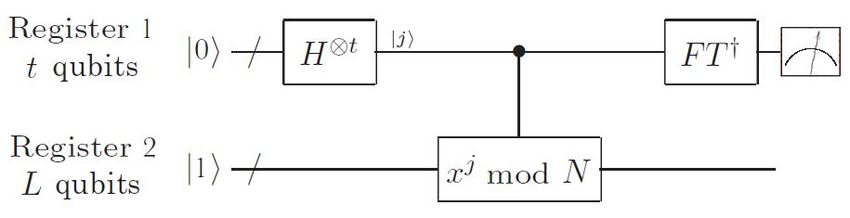
\includegraphics[width=0.6\textwidth]{figures/order-finding-circuit.png}
  \caption{Order-finding algorithm \cite{unknown}}
\end{figure}

\subsubsection{The continued fraction expansion}
우리가 앞의 알고리즘을 통해서 얻은 결과는 $s/r$이다. 따라서 이 결과로부터 $r$의 값을 얻어내는 추가적인 후처리가 필요하다. 우리가 얻은 $\varphi \approx s/r$은 임의의 $2L+1$ bit 소수이므로 임의의 실수이지만, 실제로 우리가 얻고자 하는 값은 $s/r$은 분명히 \textit{유리수}이다. 
이 특징을 활용하기 위해 continued fraction이라는 개념을 도입한다. continued fraction은 주어진 실수를 연분수 형태로 표현한 것이다.\footnote{이때 $[a_0, \cdots, a_M]$을 $M$th convergent라고 한다.}
\begin{equation*}
\left[a_0, \ldots, a_M\right] \triangleq a_0+\frac{1}{a_1+\dfrac{1}{a_2+\dfrac{1}{a_3+\ldots}}}
\end{equation*}
주어진 convergent를 연분수 형태로 변환하는 알고리즘을 \textit{continued fraction algorithm}이라고 한다.
\begin{theorem}
  $s/r$이 유리수이고, $\varphi$가 QPE로 얻은 근사값일 때 두 값의 차이가 다음과 같은 upper bound를 만족한다면, continued fraction algorithm을 적용하여 얻은 결과가 바로 $s/r$이다.
  $$ \left|\frac{s}{r}-\varphi\right| \leq \frac{1}{2 r^2} $$
\end{theorem}

Order-finding problem에서는 $(1-\delta)/r$의 높은확률로 $2L+1$ bit 정확도를 달성하기에, 다음을 만족한다.
\begin{equation*}
  \left|\frac{s}{r}-\varphi\right| \leq \frac{1}{2^{2 L+1}} \leq \frac{1}{2 r^2}
\end{equation*}
따라서 continued fraction algorithm을 적용할 수 있으므로, $O(L^3)$의 time complexity로 $s/r$을 구할 수 있고 $\gcd(s, r) =1$\footnote{만약 두 수 사이에 공약수가 존재하면, continued fraction algorithm이 반환하는 값이 통분한 값이 된다}이라면 $r$을 구할 수 있다. 
\subsubsection{Performance}
Order-finding algorithm의 정확도를 분석하기 위해서, 이 알고리즘이 실패하는 경우를 분석해보자.
\begin{itemize}
  \item QPE가 실패하는 경우 : 아주 작은 확률 $\epsilon$로 실패할 수 있다. 이 경우 qubit의 개수를 늘려서 QPE의 정확도를 높히거나 QPE를 여러번 반복하여 각 outcome의 확률을 비교하여 해결할 수 있다.
  \item $\gcd(s,r) \ne 1$인 $s$를 얻는 경우 : $0 \le s <r-1$ 범위에서 두 수가 서로소일 확률은 매우 높기 떄문에, 알고리즘을 $2 \log N$번 반복하면 이 문제를 해결할 수 있다.
\end{itemize}
\vspace{1em}
마지막으로 Order-finding algorithm의 circuit이 필요로하는 자원을 분석해보자.
\begin{itemize}
  \item $O(L)$ : Register 1에 $H$ 변환을 가하는데 필요한 circuit의 개수
  \item $O(L^2)$ : IQFT를 적용하는데 필요한 circuit의 개수
  \item $O(L^3)$ : Controlled unitary; modular exponentiation에 필요한 circuit의 개수
  \item $O(L^3)$ : continued fraction algorithm이 사용하는 time complexity
  \item $O(\log N)$ : 오류가 발생했을 때, 다시 알고리즘을 실행하는 횟수
\end{itemize}


\subsection{Shor’s algorithm: factoring}
이제 마지막으로 그 유명한 Shor's algorithm에 소개하고자 한다. Classical computer에서 polynomial time에 해결하는 효과적인 알고리즘이 아직 존재하지 않는 \textit{factoring}을 quantum computer를 사용하여 효율적으로 수행할 수 있다는 사실을 보여주는 중요한 알고리즘이다.

\vspace{1em}

Prime factorization problem은 다음과 같이 정의된다.
\begin{itemize}
  \item \texttt{input}: natural number $N$
  \item \texttt{output}: list of prime numbers $\{p_1, p_2, \dots, p_k\}$ such that $N = p_1^{e_1} \cdot p_2^{e_2} \cdot \dots \cdot p_k^{e_k}$
\end{itemize}

이를 해결하는 Shor's algorithm은 다음과 같다.
\begin{enumerate}
  \item \textbf{if} $N$이 짝수라면, \textit{return} $2$
  \item \textbf{if} $N$이 prime $p$에 대해서 $N = p^k$라면, \textit{return} $p$\footnote{이를 판단하는 효과적인 classical algorithm이 존재}
  \item $1\le x \le N-1$ 범위에서 랜덤하게 $x$를 선택한다.
  \begin{enumerate}
    \item \textbf{if} $\gcd(N, x) > 1$\footnote{using Euclidean algorithm}, \textit{return}  $\gcd(N, x)$
    \item \textbf{else}, \hyperref[sec:order-finding]{order-finding algorithm}을 사용하여 order $r$을 찾는다.
  \end{enumerate}
  \item \textbf{if} $r$이 홀수라면, \textit{goto} step 3.
  \item \textbf{else},
  \begin{enumerate}
    \item 다음을 계산한다.
    \begin{equation*}
      x^r - 1 \equiv (x^{r/2} - 1)(x^{r/2} + 1) \equiv 0 \mod N
    \end{equation*}
    \item 계산 결과로부터 얻은 2개의 항에 대해, 다음의 조건들을 확인한다.
      \begin{enumerate}
        \item \textbf{if} $N|x^{r/2}-1$, \textit{error}\footnote{order $r$이 이를 만족하는 가장 작은 수이기 때문에 이런 경우는 일어나지 않는다.}
        \item \textbf{elif} $N|x^{r/2}+1$, \textit{goto} step 3.
        \item \textbf{neither}, $N$이 $(x^{r/2}-1)(x^{r/2}+1)$을 동시에 나눌 수 없으므로 각각의 항이 $N$의 인수를 포함하고 있다는 의미이다.
        
        \textit{return} $\boxed{\gcd(N, x^{r/2}+1),\ \gcd(N, x^{r/2}+1)}$
      \end{enumerate}
  \end{enumerate}
\end{enumerate}

\vspace{0.1em}

Shor's algorithm이 성공하기 위해서는 order-finding algorithm으로 얻은 $r$이 짝수여야하며, \textbf{neither} case에 포함되어야한다. 정수론의 개념들을 도입하면, 성공확률은 $1/2$이상임을 증명할 수 있으며, 여기에서는 증명을 생략한다.

\lecture{14}{4 Nov. 10:30}{}
\section{Applications of the QFT}
이번 section에서는 QFT를 활용하는 문제들에 대해서 소개하고자 한다. QFT를 활용하여 효과적으로 해결할 수 있는 문제들은 모두 \textit{Hidden subgroup problem}으로 일반화할 수 있다.
\subsection{Period-finding}
Hidden subgroup problem을 소개하기 전에, 먼저 hidden subgroup problem의 특수한 경우들에 대해 이야기하고자 한다. 첫 번째로 소개하는 문제는 \textit{period-finding problem}이다.

\begin{itemize}
  \item \texttt{input}: period function $f$ such that $f(x) = f(x+r)$ for some \textit{unknown} integer $r,\ (0 < r < 2^L)$
  \item \texttt{output}: least integer $r>0$ such that $f(x) = f(x+r)$
\end{itemize}
주어진 period function은 \hyperref[sec:uncomputation]{uncomputation}을 사용하여 다음과 같은 unitary operator로 표현할 수 있다.
\begin{equation*}
  U_f|x\rangle|y\rangle \rightarrow|x\rangle|y \oplus f(x)\rangle
\end{equation*}

\newpage
이 $U_f$가 주어지면, 다음의 과정을 따라서 period $r$을 찾을 수 있다.
\begin{enumerate}
  \item input state : $\ket 0 \ket 0$으로 state를 초기화한다.\footnote{(1st register)함숫값을 저장하기 위해 $t = O(L + \log(1/\epsilon))$개의 qubit, (2nd register)ancilla qubit}
  \begin{equation*}
    \ket \psi = \ket 0 \ket 0
  \end{equation*}
  \item apply $H$ gate on 1st register
  \begin{equation*}
    \ket \psi = \frac{1}{\sqrt{2^t}} \sum_{x=0}^{2^t-1}\ket x \ket 0
  \end{equation*}
  \item apply $U_f$ : $\ket y = \ket 0$이므로 2nd register에 $f(x)$가 저장된다. 
  \begin{equation*}
    \ket \psi = \frac{1}{\sqrt{2^t}} \sum_{x=0}^{2^t-1}|x\rangle|f(x)\rangle 
  \end{equation*}
  \item apply QFT on \textbf{2nd} register
  
  QFT를 사용하여 함수 $f(x)$를 표현하면, 다음과 같다. (See Definition.~\ref{def:QFT})
  \begin{equation*}
    f(x) \rightarrow  \frac{1}{\sqrt{r}} \sum_{l=0}^{r-1} e^{2 \pi i l x / r}|\hat f(l)\rangle,\qquad  |\hat{f}(l)\rangle \triangleq \frac{1}{\sqrt{r}} \sum_{x=0}^{r-1} e^{-2 \pi i l x / r}|f(x)\rangle
  \end{equation*}
  따라서 이를 이용하면, state를 다음과 같이 표현할 수 있다. 
  \begin{equation*}
    \ket \psi = \frac{1}{\sqrt{r 2^t}} \sum_{l=0}^{r-1} \sum_{x=0}^{2^t-1} e^{2 \pi i l x / r}|x\rangle|\hat{f}(l)\rangle
  \end{equation*}
  \item apply IQFT on \textbf{1st} register\footnote{2nd register가 $x, l$간의 QFT를 이용했다면, 1st register는 $l$이 아닌 다른 변수 $y$에 대해 IQFT를 수행하게 된다.}
  \begin{equation}
      \ket \psi = \frac{1}{\sqrt{r} 2^t} \sum_{l=0}^{r-1} \sum_{x, y=0}^{2^t-1} e^{2 \pi i l x / r} e^{-2 \pi i x y / 2^t}|y\rangle|\hat{f}(l)\rangle =\frac{1}{\sqrt{r} 2^t} \sum_{l=0}^{r-1} \sum_{x, y=0}^{2^t-1} e^{(2 \pi i x)(l/r - y/2^t)}|y\rangle|\hat{f}(l)\rangle \label{eq:period-final}
  \end{equation}
\end{enumerate}

final state의 coefficient를 분석하기 위해 $r$이 $2^t$를 나누는가에 대한 cases를 분석할 수 있다.
\begin{itemize}
  \item $r\nmid 2^t$ : 일반적으로는 $r$이 $2^t$를 나누지 않는 경우가 더 많다.\footnote{$2^t$의 약수; 2의 거듭제곱이 아닌 이상 나눌 수 없음} 그러나 이 경우에도 최종 outcome이 높은 확률로 $nl$이 된다. 
  \item $r\mid 2^t$ : $nr  = 2^t$가 되게 만드는 positive integer가 존재한다. 따라서 이를 이용하면 state가 다음과 같이 단순화 된다. (Eq.~\eqref{eq:period-final}에 $r=2^t/n$ 대입)\footnote{$nl - y$에 대해, complex exponential의 orthogonality를 사용하여 정리한다.}
  \begin{equation*}
    \frac{1}{2^t} \sum_{x, y=0}^{2^t-1} e^{(2 \pi i x / 2^t)(nl-y)}|y\rangle=\sum_{y=0}^{2^t-1} \delta_{y, n l}|y\rangle=|n l\rangle = \frac{1}{\sqrt{r}} \sum_{l=0}^{r-1}|n l\rangle|\hat{f}(l)\rangle
  \end{equation*}
  따라서 1st register를 측정한 결과를 $2^t$로 나누면 $nl/2^t = l/r$이므로 $r$을 구할 수 있다. $\Box$
\end{itemize}

\subsection{Discrete logarithm}
이번에 소개하려는 문제는 \textit{Discrete logarithm problem}; 이산 로그 문제이다. 이 문제는 다과 같이 정의된다.
\begin{itemize}
  \item \texttt{input}: $x \in G$, 이때 $G = \langle g \rangle$는 $g$로부터 만들어지는 cyclic group\footnote{See \url{https://en.wikipedia.org/wiki/Cyclic_group}}\footnote{대표적인 cyclic group으로 modular multiplication이 있다.}이다.
  \item \texttt{output}: minimum $\alpha$ such that $g^\alpha = x$ (or equivalently, $\alpha = \log_g x$)
\end{itemize}
\vspace{1em}
다음은 다양한 cyclic group들의 discrete log에 대한 예시이다.
\begin{itemize}
  \item (Property of logarithm) For any $G=\langle g\rangle, \log _g 1=0$,
  \item For $G=\mathbb{Z}_7^{\times}, \log _3 2=2$,
  \item For $G=\mathbb{Z}_{541}^{\times}, \log _{126} 282=101$.
\end{itemize}

이 문제를 해결하기 위해, Discrete logarithm problem을 \textit{period finding} problem의 형태로 변환할 수 있다.
먼저 다음 integer function $f$를 가정하자. 여기서 $\gcd(a, N) = 1$이며, modulo $N$에서 $a$ order가 $r$이라고 하자. 
\begin{equation*}
  f\left(x_1, x_2\right)=a^{s x_1+x_2} \bmod N
\end{equation*}
이렇게 정의한 함수는 어떤 $l$에 대해 $(l, -ls)$라는 period를 가진다.
\begin{equation*}
  f(x_1+l, x_2-ls)=a^{sx_1 + sl + x_2 - ls} \mod N \equiv a^{sx_1 + x_2} \mod N = f(x_1, x_2)
\end{equation*}
Uncomputation을 사용하면 이 $f$에 대응되는 unitary를 구성할 수 있다.
\begin{equation*}
  U\left|x_1\right\rangle\left|x_2\right\rangle|y\rangle=\left|x_1\right\rangle\left|x_2\right\rangle|y \oplus f(x)\rangle
  \end{equation*}
우리는 discrete logarithm problem을 다시 다음과 같이 표현할 수 있다.\footnote{$a$가 $g$, $s$가 $\alpha$에 대응된다.}
\begin{itemize}
  \item \texttt{input}: $b \in \mathbb Z_N^\times$ such that $b \equiv a^s \mod N$, $a \in \mathbb Z$
  \item \texttt{output}: integer $s$
\end{itemize}

따라서 period function $f$를 이용하면 문제를 해결할 수 있다. 
\begin{enumerate}
  \item input state : 3개의 register를 사용한다.
  \begin{equation*}
    \ket \psi = \ket 0 \ket 0 \ket 0
  \end{equation*}
  \item apply $H$-gate on 1st and 2nd register
  \begin{equation*}
    \ket \psi = \frac{1}{2^t} \sum_{x_1, x_2=0}^{2^t-1}\left|x_1\right\rangle\left|x_2\right\rangle|0\rangle
  \end{equation*}
  \item apply $U_f$ : $f(x_1, x_2)$를 3rd register에 저장한다.
  \begin{equation*}
    \ket \psi = \frac{1}{2^t} \sum_{x_1, x_2=0}^{2^t-1}\left|x_1\right\rangle\left|x_2\right\rangle\left|f\left(x_1, x_2\right)\right\rangle
  \end{equation*}
  \item apply QFT on 3rd register 
  
  QFT를 사용하여 함수 $f(x_1, x_2)$를 표현하면 다음과 같다. (See Definition.~\ref{def:QFT})
  \begin{equation*}
    \left|f\left(x_1, x_2\right)\right\rangle \rightarrow \frac{1}{r} \sum_{l_1, l_2=0}^{r-1} e^{2 \pi i\left(l_1 x_1+l_2 x_2\right) / r}|\hat{f}\left(l_1, l_2\right)\rangle 
  \end{equation*}
  \begin{equation*}
    |\hat{f}\left(l_1, l_2\right)\rangle \triangleq \frac{1}{r} \sum_{x_1, x_2=0}^{r-1} e^{-2 \pi i\left(l_1 x_1+l_2 x_2\right) / r}\left|f\left(x_1, x_2\right)\right\rangle=\frac{1}{\sqrt{r}} \sum_{j=0}^{r-1} e^{-2 \pi i l_2 j / r}|f(0, j)\rangle
  \end{equation*}
  따라서 이를 이용하면, state를 다음과 같이 표현할 수 있다.\footnote{put $l_1 = l_2, l_2 = sl_2$}
  \begin{align*}
    \ket \psi &= \frac{1}{2^t \sqrt{r}} \sum_{l_2=0}^{r-1} \sum_{x_1, x_2=0}^{2^t-1} e^{2 \pi i\left(s l_2 x_1+l_2 x_2\right) / r}\left|x_1\right\rangle\left|x_2\right\rangle|\hat{f}\left(s l_2, l_2\right)\rangle  \\ 
    &=\frac{1}{2^t \sqrt{r}} \sum_{l_2=0}^{r-1}\left[\sum_{x_1=0}^{2^t-1} e^{2 \pi i\left(s l_2 x_1\right) / r}\left|x_1\right\rangle\right]\left[\sum_{x_2=0}^{2^t-1} e^{2 \pi i\left(l_2 x_2\right) / r}\left|x_2\right\rangle\right]|\hat{f}\left(s l_2, l_2\right)\rangle
  \end{align*}
  \item apply IQFT on 1st and 2nd register
  \begin{equation*}
    \ket \psi = \frac{1}{\sqrt{r}} \sum_{l_2=0}^{r-1}\left|s l_2 / r\right\rangle\left|l_2 / r\right\rangle|\hat{f}\left(s l_2, l_2\right)\rangle
  \end{equation*}
\end{enumerate}

따라서 1st, 2nd register를 측정하면 각각 $sl/r$, 그리고 $l/r$이라는 값을 얻게 되는데, $sl/r \times r/l = s$이므로 $s$를 구할 수 있다. $\Box$  

\subsection{Hidden subgroup problem}
이제 Hidden subgroup problem에 대해 이야기할 시간이 찾아왔다.\footnote{See \url{https://en.wikipedia.org/wiki/Hidden_subgroup_problem}}
\begin{definition}[Hidden subgroup problem]
  Let $f$ be a function from finitely generated group $G$ to some finite set $X$. s.t. $f$ is constant on the cosets of a subgroup $K$, and distinct on each coset.\footnote{$K$가 주어졌을 때, coset은 $G$의 원소에 대해서 $gK = \{gk : k \in K\}$로 정의된다.}\footnote{같은 coset이라면 $f$의 값은 매우 동일하지만, 서로 다른 coset에 속한다면 $f$의 값은 서로 다르다.}
  \begin{equation*}
    f: G \rightarrow X \quad  \longrightarrow \quad U_f\ket g \ket h = \ket g \ket{h \oplus f(g)} \quad (\text{for } g \in G, h \in X)
  \end{equation*}
  \textit{Find a generating set for} $K$.
\end{definition}

앞에서 우리가 다루었던 order-finding problem, period-finding, discrete logarithm과 같은 문제들이 Hidden subgroup problem의 특수한 예시이다. 예를 들어, order-finding problem이 왜 Hidden subgroup problem으로 표현될 수 있는지 알아보자.
Hidden subgroup problem에서 각각을 다음과 같이 정의하자.
\begin{itemize}
  \item $G = \mathbb Z$
  \item $K = r\mathbb Z$
  \item (coset) $K_g = \{rg\}$ for $g \in \mathbb Z$ (e.g., $K_1 = \{\cdots, -2, -1, 0 \cdots, 1, 2\}, K_3 = \{\cdots, -6, -3, 0 \cdots, 3, 6\}$ )
  \item $f(k)  = a^k \mod N$
\end{itemize}
이때, (1) $f(k) = f(k+r)$의 주기를 가지고 (2) $0 \leq k \leq r-1$ 범위에서 각각의 $f(k)$의 값은 모두 구분된다. 
이 두 가지 성질은 $f$가 동일한 coset에 속하는 원소들에 대해서 constant하고, 서로 다른 coset에 속한 원소들에 대해서는 distinct한 값을 가지는 것을 의미한다. 따라서 order-finding problem은 Hidden subgroup problem의 특수한 경우로 생각할 수 있다.

$G$가 finite abelian group\footnote{교환법칙이 성립하는 군}이라면, QFT를 적용하여 Hidden subgroup problem을 해결할 수 있다. 그러나, non-abelian group에 대해서는 아직 이 문제를 효과적으로 푸는 방법이 알려지지 않았다. (non-abelian group에 대한 대표적인 문제가 바로 \textit{Graph isomorphism})

\section{Quantum search algorithms}
Quantum search algorithm에 대해서 알아보자. 정렬되어있거나 특정한 규칙이 있는 데이터에 대한 search algorithm은 classical computer에서도 이미 충분히 효과적으로 수행할 수 있다. 그러나, 여기에서 다룰 search problem은 \textit{unstructured}한 데이터를 다룬다.
이를 위해 먼저 하나의 oracle을 가정하자. 

$N$개의 항목이 있는 unstructured 데이터에 대해서, $f(x)$는 $x$번째 항목이 우리가 찾고자 하는 항목인지를 판단하는 oracle이다. 따라서 $f(x) = 1$이면, $x$가 solution이 되고 $f(x) =0$이면, $x$가 solution이 아니다.
편의를 위해서 $N=2^n$이며, 찾고자 하는 항목의 개수가 $M$ ($1 \le M \le N$)이라고 가정하자. 

\begin{equation*}
  f : \{0, 1\}^n \rightarrow \{0, 1\}
\end{equation*}

이 문제를 어떻게 해결할 수 있을까? 단순하게 생각하면 랜덤한 $x$를 선택하여 $f(x)$의 값을 확인한 뒤 $x$가 solution인지 아닌지를 판단할 수 있으며, 선택한 $x$가 solution일 확률은 $M/N$이다. 만약 $N$이 $M$에 비해 exponential하게 크다면, success probability는 exponential하게 줄어들기에 이는 효율적이지 않다. 

Quantum computer에서 $f$에 대한 unitary는 다음과 같이 정의된다.
\begin{equation*}
  |x\rangle|q\rangle \xrightarrow{O}|x\rangle|q \oplus f(x)\rangle
\end{equation*}
$x$는 $N$개의 항목에 대한 인덱스를 나타내기 위해 $n$개의 qubit으로 이루어지며, query qubit은 1개의 qubit으로 이루어진다. 즉, 만약 $f(x) = 1$; $x$가 solution이라면 query qubit의 값이 bit-flip된다.

만약 $\ket q = \ket -$으로 설정하면, 다음과 같은 일이 벌어진다.
\begin{equation*}
  |x\rangle\left(\frac{|0\rangle-|1\rangle}{2}\right) \xrightarrow{O} \frac{|x\rangle|f(x)\rangle-|x\rangle|1 \oplus f(x)\rangle}{2}=(-1)^{f(x)}|x\rangle\left(\frac{|0\rangle-|1\rangle}{2}\right)
\end{equation*}
$x$가 solution이라면 bit-flip이 일어나서 phase가 바뀌게 되고, solution이 아닌 경우에는 phase가 바뀌지 않는다. 따라서 이 oracle $O$를 다음과 같이 단순하게 쓸 수 있다.
\begin{equation*}
  |x\rangle \xrightarrow{O}(-1)^{f(x)}|x\rangle .
\end{equation*}

따라서 이 oracle을 활용하면, classical computer와 동일한 randomized algorithm을 적용하여도 $O(\sqrt{N/M})$의 complexity를 가진다.


\subsection{Grover operator}
Unstructured search problem을 $\Theta(\sqrt N)$ 복잡도로 해결할 수 있는 Grover search algorithm을 설명하기 위해 먼저 \textit{Grover operator} $G$를 정의한다.\footnote{$G = (H^{\otimes n}(2|0\rangle\langle 0|^{\otimes n}-I) H^{\otimes n})O$}
\begin{equation*}
  G \triangleq (2|\Psi\rangle\langle\Psi|-I) O
\end{equation*}
이때 $\ket{\Psi}$는 다음과 같이 정의되며\footnote{$N$까지의 모든 가능한 입력들의 superposition}, $O$는 oracle이다.
\begin{equation*}
  |\Psi\rangle=\frac{1}{\sqrt{N}} \sum_{x=0}^{N-1}|x\rangle,
\end{equation*}

우리는 이제 $G$가\textit{superposition of solutions} state $\ket \beta$, \textit{superposition of non-solutions} $ket alpha$가 span하는 two-dimensional space에서 회전 연산을 수행한다는 것을 보일 것이다.
\begin{equation}
  |\alpha\rangle \triangleq \frac{1}{\sqrt{N-M}} \sum_{x: f(x) = 0}|x\rangle, \quad|\beta\rangle \triangleq \frac{1}{\sqrt{M}} \sum_{x: f(x) = 1}|x\rangle . \label{def:solution-state}
\end{equation}
$\ket \Psi$를 다음과 같이 $\ket \alpha, \ket \beta$의 linear combination으로 표현할 수 있기때문에, $\ket{\Psi}$는 $\text{span}\{\ket \alpha, \ket \beta \}$ vector space에 속한다. 
\begin{equation*}
  |\Psi\rangle=\sqrt{\frac{N-M}{N}}|\alpha\rangle+\sqrt{\frac{M}{N}}|\beta\rangle
\end{equation*}

$G$가 수행하는 연산을 이해하기 위해서, 각 단계마다 gate가 수행하는 역할을 분석해보자.
\begin{enumerate}
  \item Oracle $O$가 $\text{span}\{\ket \alpha, \ket \beta \}$에 속하는 임의의 vector에 대해 다음과 같이 동작한다.
  \begin{equation*}
    O(a|\alpha\rangle+b|\beta\rangle)=a|\alpha\rangle-b|\beta\rangle
  \end{equation*}
  $\Rightarrow$ $\ket \alpha$ 축에 대한 \textit{reflection}
  \item ($2 \ket \Psi \bra \Psi - I$) 연산은 eigenvalue $\pm 1$에 대해 spectral decomposition을 할 수 있다.
  \begin{equation*}
    2 \ket \Psi \bra \Psi - I = \ket \Psi \bra \Psi  - (I - \ket \Psi \bra \Psi)
  \end{equation*}
  $\ket \Psi \bra \Psi$는 $\ket \Psi$에 대한 projector이고 반대로 $I - \ket{\Psi} \bra{\Psi}$는 $\ket \Psi$의 \textit{orthogonal subspace}에 대한 projector이다.
  따라서 이 연산은 $\{\ket \Psi, \ket \Psi^\perp\}$ vector space에서 $\ket \Psi$ 축에 대한 reflection을 수행하게 된다. 
  
  $\Rightarrow$ $\ket \Psi$ 축에 대한 \textit{reflection}
\end{enumerate}

따라서 2개의 reflection operator들의 곱으로 정의되는 Grover operator는 \textbf{rotation} operator가 된다.
이는 $G^k\ket{\Psi}$를 수행하면 $\text{span}\{\ket \alpha, \ket \beta \}$ vector space에 속하는 모든 vector를 만들어 낼 수 있다는 의미이다!

\vspace{1em}

좀 더 자세한 설명을 위해 $\ket{\Psi}$를 $\theta$를 사용하여 표현하자.\footnote{$(\sqrt{(N-M)/N})^2 + (\sqrt{M/nN})^2 = 1$을 이용하면 $\cos, \sin$ function을 이용할 수 있다.}
\begin{equation*}
  |\Psi\rangle=\cos \frac{\theta}{2}|\alpha\rangle+\sin \frac{\theta}{2}|\beta\rangle
\end{equation*}
그럼, $G$가 $\ket{\Psi}$에 대해 가해지면, state는 다음과 같이 변한다.

$\Rightarrow$ 즉, $G$는 $\ket \Psi$를 $\theta$만큼 rotation 시킨다.
\begin{equation}
  G|\Psi\rangle=\cos \frac{3 \theta}{2}|\alpha\rangle+\sin \frac{3 \theta}{2}|\beta\rangle
\end{equation}

따라서 $G$ gate는 $\{\ket \alpha, \ket \beta\}$ basis에 대해 다음과 같은 matrix notation으로 표현할 수 있다.
\begin{equation*}
  G=\left(\begin{array}{cc}
    \cos \theta & -\sin \theta \\
    \sin \theta & \cos \theta
    \end{array}\right)
\end{equation*}
$G$를 $k$번 적용하면, 다음 상태를 얻게된다.
\begin{equation*}
  G^k|\Psi\rangle=\cos \left(\frac{2 k+1}{2} \theta\right)|\alpha\rangle+\sin \left(\frac{2 k+1}{2} \theta\right)|\beta\rangle
\end{equation*}
만약 $(2^k+1 / 2)\theta$가 $\pi/2$에 충분히 가깝다면, $\cos((2k+1/2) \theta)$가 0에 가까워지기 떄문에 $G^k|\Psi\rangle$를 측정하면, $\ket \beta$를 얻을 확률이 높아진다.
이 아이디어를 기반으로 Grover search algorithm이 제안되었다.

\begin{figure}
  \centering
  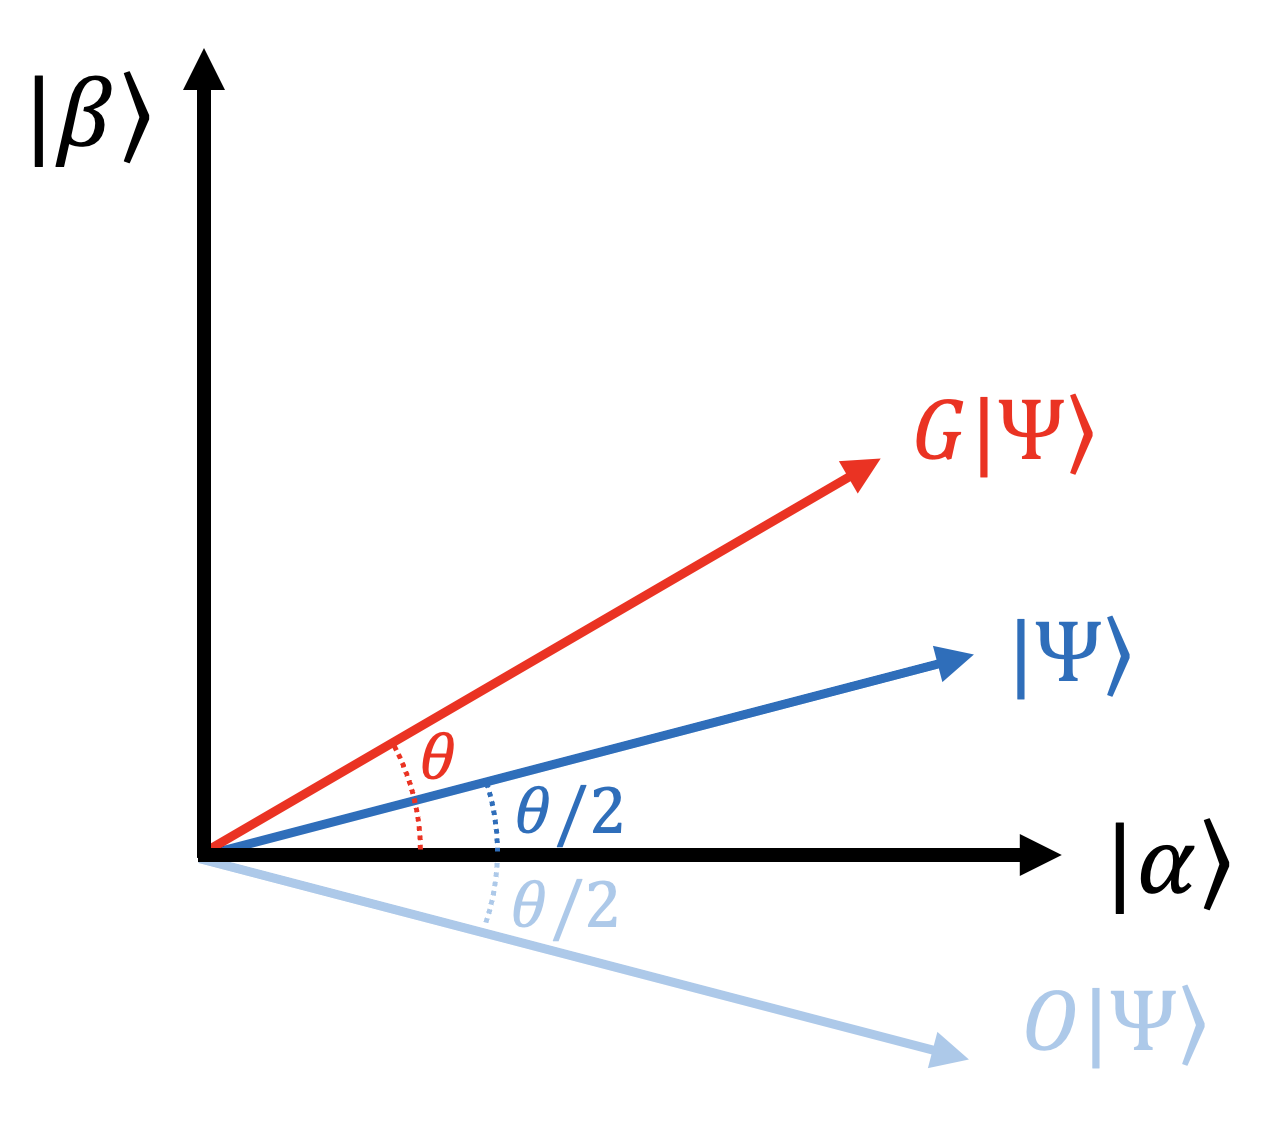
\includegraphics[width=0.35\linewidth]{figures/grover.png}
  \caption{Grover operator}
  \label{fig:grover-operator}
\end{figure}

\vspace{1em}

\subsection{Grover search algorithm}
Grover search algorithm은 앞에서 도입한 Grover operator를 사용하여 unstructured search problem을 해결하는 알고리즘으로, 다음과 같은 과정을 따른다.
\begin{enumerate}
  \item input state 
  \begin{equation*}
    \ket \psi = \ket 0^{\otimes n}
  \end{equation*}
  \item apply Hadamard gate : $\ket \Psi$를 만들기 위해 Hadamard gate를 적용한다.
  \begin{equation*}
    \ket \psi = \frac{1}{\sqrt N} \sum_{x=0}^{N-1}\ket x
  \end{equation*}
  \item (Grover iteration; $G = (H^{\otimes n}(2|0\rangle\langle 0|^{\otimes n}-I) H^{\otimes n})O$) 다음을 $k$번 반복한다.
  \begin{enumerate}
    \item apply the oracle $O$
    \item apply the Hadamard gate $H^{\otimes n}$
    \item perform a conditional phase shift ($0$이 아닌 모든 basis는 phase shift가 된다.)
    \begin{equation*}
      |x\rangle \rightarrow-(-1)^{\delta_{x 0}}|x\rangle 
    \end{equation*}
    \item apply the Hadamard gate $H^{\otimes n}$
  \end{enumerate}
  \item measure the state : 우리가 찾고자하는 $M$개의 항목중에서 하나의 idex를 확률에 따라 얻을 수 있다. (See Eq.~\eqref{def:solution-state})
  \begin{equation*}
    \ket \psi = \cos \left(\frac{2 k+1}{2} \theta\right)|\alpha\rangle+\sin \left(\frac{2 k+1}{2} \theta\right)|\beta\rangle \longrightarrow \ket{\beta}
  \end{equation*}
\end{enumerate}


\begin{figure}[h]
  \centering
  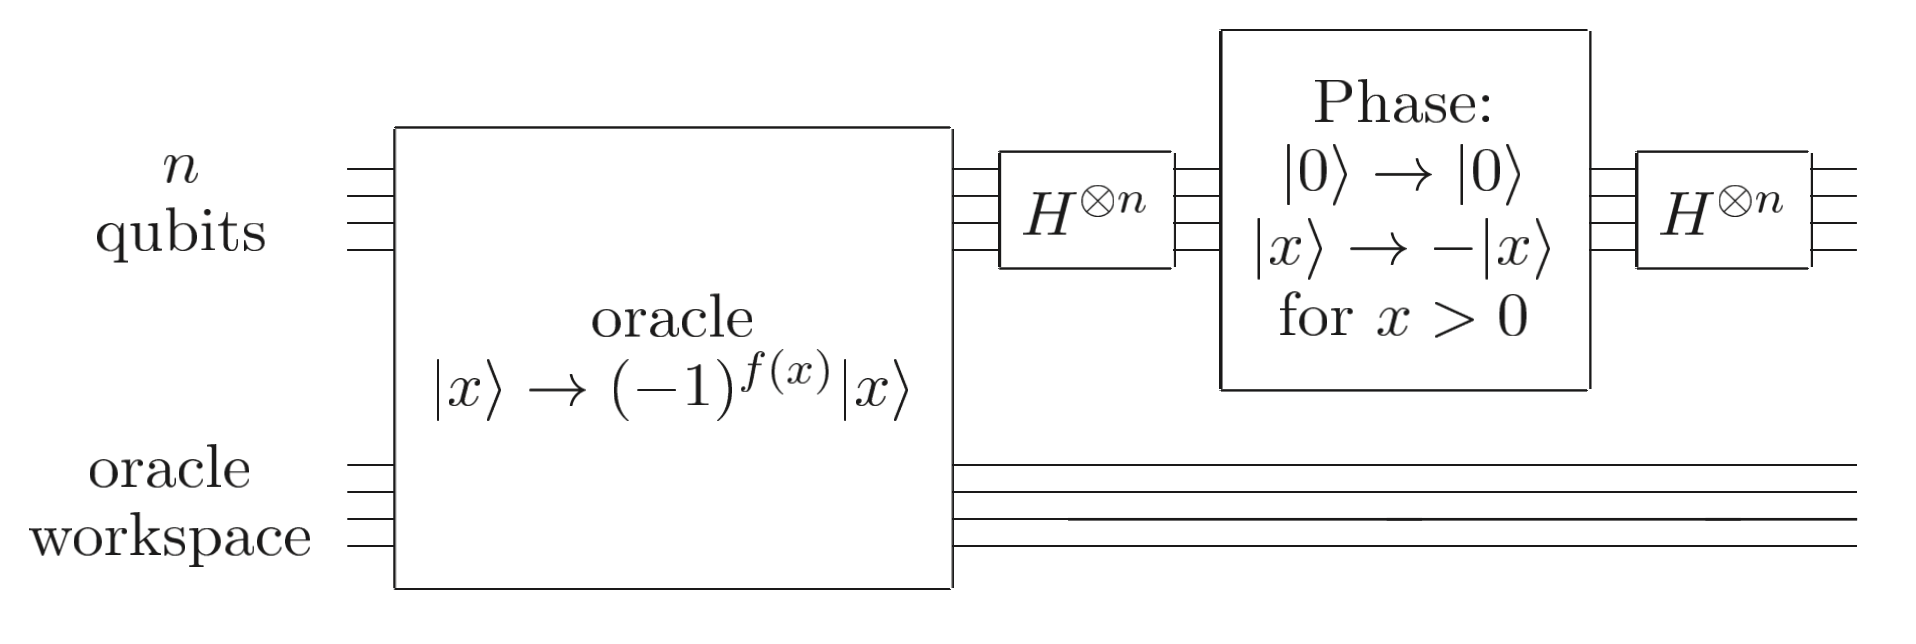
\includegraphics[width=0.6\linewidth]{figures/Grover_operator.png}
  \caption{Grover operator circuit}
  \label{fig:grover-operator-circuit}
\end{figure}

\begin{figure}[h]
  \centering
  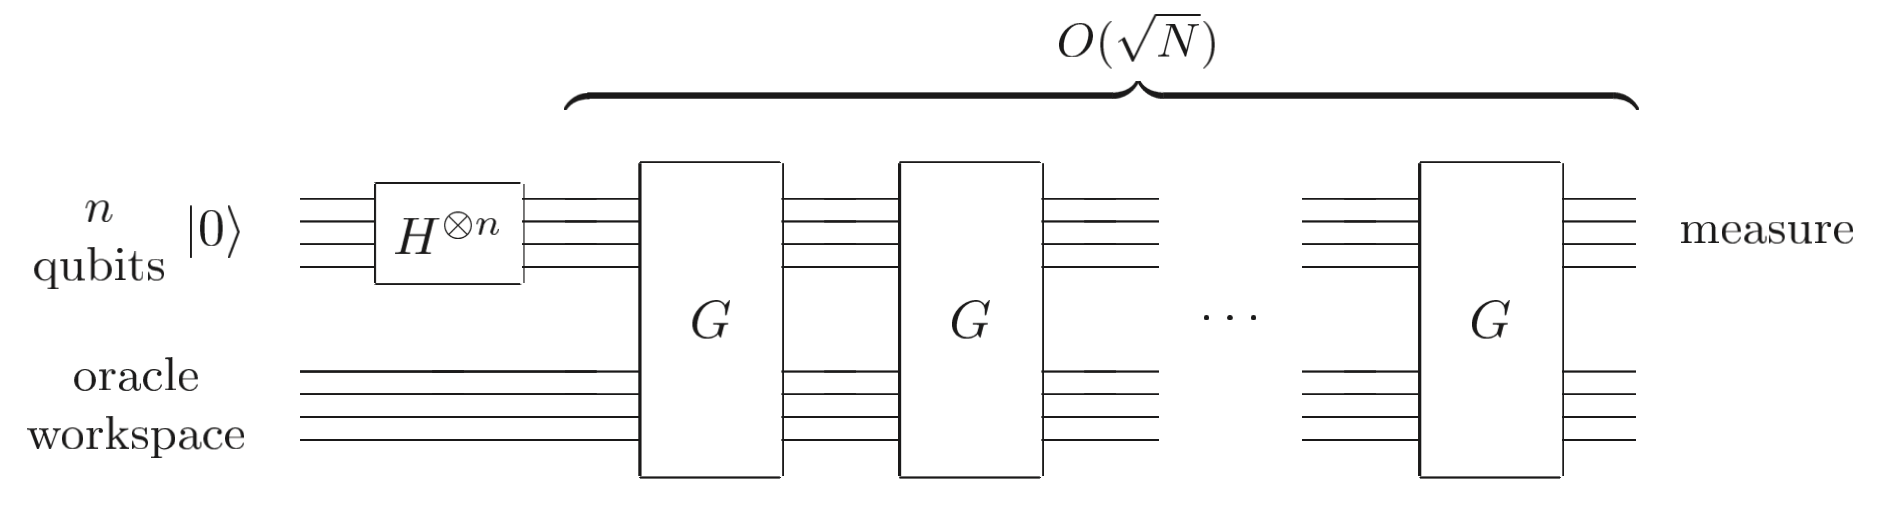
\includegraphics[width=0.65\linewidth]{figures/Grover_circuit.png}
  \caption{Grover search algorithm circuit}
  \label{fig:grover-search-circuit}
\end{figure}

\subsection{Performance}
그렇다면, Grover algorithm을 사용하여 solution state $\ket \beta$에 다가가기 위해서는 총 몇 번의 iteration이 필요할까?
Iteration을 $k$번 했을 때, state는 다음과 같다.
\begin{equation*}
  G^k|\Psi\rangle=\cos \left(\frac{2 k+1}{2} \theta\right)|\alpha\rangle+\sin \left(\frac{2 k+1}{2} \theta\right)|\beta\rangle
\end{equation*}
$k$를 다음과 같이 설정하면 $\ket \alpha$의 amplitude가 0이 되므로, state가 $\ket \beta$가 된다.
\begin{equation*}
  \frac{2 k+1}{2} \theta=\frac{\pi}{2}
\end{equation*}
위 조건에 가장 가까운 $k$를 선택했을 때, 얻을 수 있는 최종 state $\ket \psi$의 각도는 $\theta / 2 \leq \pi / 4$로 bound 된다. 따라서 최종 state가 $\beta$가 될 확률은 적어도 절반이 넘는다.\footnote{$\sin(\pi/4) = \cos(\pi/4) = 1/\sqrt{2}$}

좀 더 구체적으로 나타내면 다음과 같다.\footnote{$\arccos \sqrt{1-x} \approx \sqrt{x}+O\left(x^{3 / 2}\right)$ 임을 이용한다.}
\begin{equation*}
  k=\frac{\pi}{2 \theta}-\frac{1}{2}=\frac{\pi}{4 \arccos \sqrt{(N-M) / N}}-\frac{1}{2}=\frac{\pi}{4} \sqrt{\frac{N}{M}}-\frac{1}{2}-O\left(\sqrt{\frac{M}{N}}\right)
\end{equation*}

따라서 Grover search algorithm의 complexity; $k$는 $O(\sqrt{N/M})$이다. 이는 랜덤하게 $M$을 선택하여 문제를 해결하는 방법보다 훨씬 효율적이다. ($O(N/M)$\footnote{성공확률이 $M/N$이므로, complexity는 그 역수})

한 가지 남아있는 문제점은, $k$를 선택하기 위해서는 $M$의 값을 알아야한다는 것이다. 
만약 문제에서 우리가 찾으려는 항목이 있는 곳의 개수 $M$을 제공하지 않는다면, $k$를 결정할 수 없다. 이를 해결하는 2가지 방법이 존재한다.
\begin{itemize}
  \item $k$를 랜덤하게 선택하여 탐색한다. (이 경우에도 비슷한 수준의 성능을 낼 수 있음이 알려져있다.)
  \item $M$을 추정하는 알고리즘을 사용한다. (by \hyperref[sec:amplitude-estimation]{amplitude estimation algorithm})
\end{itemize} 

\lecture{15}{6 Nov. 10:30}{}
\subsection{Example: Classical circuit-SAT problem}
이번에는 Grover search algorithm을 이용하여 classical circuit-SAT problem을 해결하는 예시를 살펴보자. 

\textbf{Problem} Boolean function $f: \{0, 1\}^n \rightarrow \{0, 1\}$을 계산하는 Poly($n$) 크기의 classical circuit이 존재한다고 가정하자. 
이떄, $f(x) = 1$이 되도록 만드는 $x$가 존재하는가? 존재한다면 $x$는 몇 개인가?

\vspace{1em}
랜덤하게 $x$를 결정하여 $f(x)$의 값을 확인하는 방식은 $O(2^n)$이라는 complexity를 가진다.
그러나 Grover search algorithm을 사용하면, $O(2^{2/n})$이라는 complexity만으로도 이 문제를 해결할 수 있다. 

\vspace{1em}
먼저 uncomputation을 사용하여 주어진 $f$에 대한 $O_f$를 설계하자.
\begin{equation*}
  O_f|x, b\rangle=|x, b \oplus f(x)\rangle
\end{equation*}
이 oracle은 $N$개의 항목중에서 $M$개의 항목을 찾기 위해 각 항목의 위치가 우리가 찾기를 바라던 값인지를 확인하는 search algorithm의 oracle과 동일하다.
따라서 Graver search algorithm을 동일한 방식으로 적용하면 주어진 문제를 쉽게 해결할 수 있다.

\subsection{Example: Amplitude amplification}\label{sec:amplitude-amplification}
Grover search algorithm은 \textit{amplitude amplification}을 수행하기 위해 사용할 수 있다. Amplitude amplification은 bad state $\ket \alpha$에 대한 amplitude는 감소시키고, good state $\ket \beta$에 대한 amplitude는 증가시키는 것을 목적으로 한다.
먼저 다음과 같은 unitary를 가정하자.\footnote{amplitude amplification은 사실 unstructured search problem에 대한 일반화된 형태이다.}
\begin{equation*}
  \left|\psi_0\right\rangle \triangleq U\left|0^n\right\rangle =\sqrt{p_0}|\beta\rangle+\sqrt{1-p_0}|\alpha\rangle =\sin \frac{\theta}{2}|\beta\rangle+\cos \frac{\theta}{2}|\alpha\rangle, \qquad s.t. \  \langle\alpha |  \beta\rangle=0, p_0 \ll 1
\end{equation*}
이 문제에서는 unstructured search problem에서 요구하는 $\ket \alpha, \ket \beta$가 각각 특정 computational basis의 superposition state여야한다는 조건이 없기 때문에, $\ket \alpha$에 대한 reflector를 설계해야한다.

\vspace{1em}

$U, U^\dagger$ 그리고 bad state $\ket \alpha$의 orthogonal subspace에 대한 projector $I - \ket \alpha \bra \alpha$가 주어졌을 때, 다음과 같이 initial state $\ket{\psi_0}$의 orthogonal subspace에 대한 projector $I - \ket {\psi_0} \bra {\psi_0}$를 만들어낼 수 있다.
\begin{equation*}
2\left|\psi_0\right\rangle\left\langle\psi_0\right|-I=U\left(2\left|0^n\right\rangle\left\langle 0^n\right|-I\right) U^{\dagger} .
\end{equation*}
따라서 다음 연산을 수행하면, $G$ operator와 유사하게, $\ket \alpha$에 대한 reflection, $\ket{\psi_0}$에 대한 reflection이 일어나서 $\ket beta$에 가깝게 회전하게 된다.
\begin{equation*}
  G \triangleq (2\ket{\psi_0}\bra{\psi_0} - I)(2 \ket{\alpha}\bra{\alpha} - I) = U\left(2\left|0^n\right\rangle\left\langle 0^n\right|-I\right) U^{\dagger}(2|\alpha\rangle\langle\alpha|-I)
\end{equation*}

\section{Amplitude estimation algorithm (Quantum counting)}\label{sec:amplitude-estimation}
Amplitude estimation algorithm; Quantum counting algorithm은 Grover search problem에서 solution의 개수 $M$을 추정하는 알고리즘이다.
이 알고리즘을 먼저 사용하게 되면, $M$이 얼마인지 추정할 수 있을뿐더러 만약 주어진 데이터셋에 solution이 존재하지 않는 경우, $M=0$임을 확인해줄 수 있다.

이를 이용하면, search problem의 해가 있는지 없는지를 판단하는 문제의 형태로 변환할 수 있는 NP-complete 문제를 푸는데 도움이 될 수 있다.

\vspace{1em}

Grover operator $G$를 $\{\ket \beta, \ket \alpha\}$에 대해서 matrix 표현으로 나타내면, 다음과 같다.
\begin{equation*}
  \left(\begin{array}{cc}
    \cos \theta & \sin \theta \\
    -\sin \theta & \cos \theta
    \end{array}\right)
\end{equation*}
$G$를 spectral decomposition하면 다음과 같이 나타낼 수 있고
\begin{equation*}
  G=\cos \theta|\beta\rangle\langle\beta|+\cos \theta|\alpha\rangle\langle\alpha|+\sin \theta|\beta\rangle\langle\alpha|-\sin \theta|\alpha\rangle\langle\beta| .
\end{equation*}
따라서 $G$의 eigenvalue, eigenvector는 각각 다음과 같다.
\begin{itemize}
  \item eigenvalue : $e^{\pm i {\color{red} \theta}}$
  \item eigenvector : $\ket{\psi_{\pm}} = \frac{1}{\sqrt{2}}(|\beta\rangle \pm i|\alpha\rangle)$
\end{itemize}

만약 우리가 $e^{\pm i \theta}$에서 $\theta$의 값을 알아낸다면 $\sin(\theta/2) = \sqrt{M/N}$이므로 $M$이 얼마인지 추정할 수 있다. $\theta$의 값을 알아내기 위해 \hyperref[sec:QPE]{phase estimation}을 도입할 수 있다. 그런데 $G$의 eigenvector를 준비하려면, $\ket \alpha, \ket \beta$의 상태를 알아야한다는 문제가 존재한다.

\begin{figure}[H]
  \centering
  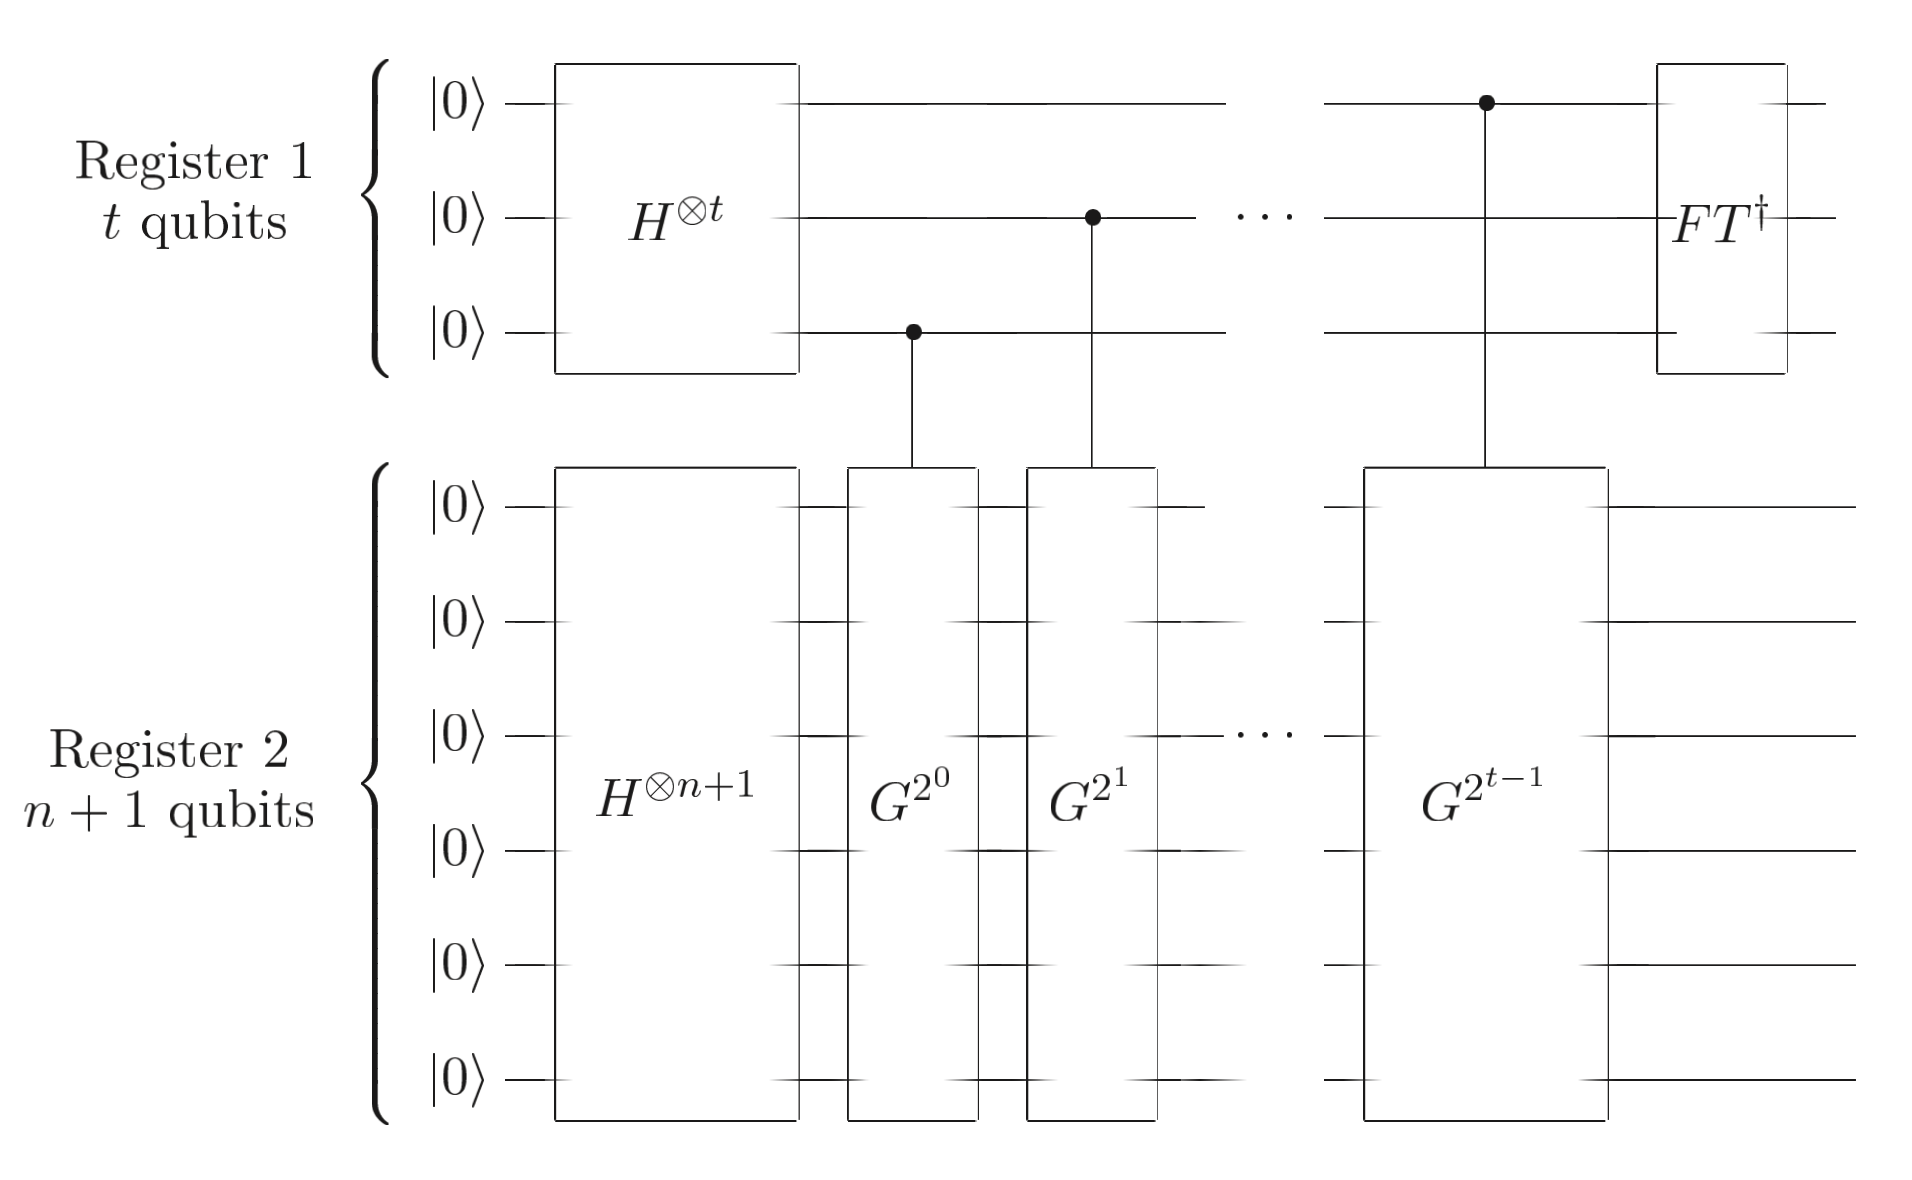
\includegraphics[width=0.6\linewidth]{figures/quantum_counting.png}
  \caption{Quantum counting circuit}
  \label{fig:amplitude-estimation}
\end{figure}


이를 해결하기 위해 initial state와 $G$의 eigenvector가 다음의 관계를 가짐을 이용하자.
\begin{equation*}
  \left|\left\langle\psi_0 | \psi_{+}\right\rangle\right|^2=\frac{1}{2}\left|\sin \frac{\theta}{2}+i \cos \frac{\theta}{2}\right|^2=\frac{1}{2}=\left|\left\langle\psi_0 | \psi_{-}\right\rangle\right|^2 .
\end{equation*}
즉, eigenvector 대신에 initial state를 이용하면, 각각 $1/2$의 확률로 eigenstate 둘 중 하나가 되기 때문에 이를 이용하여 $\theta$를 추정할 수 있다. Fig.~\ref{fig:amplitude-estimation}에서 Register 2를 $\ket{\psi_0}$으로 초기화하기 위해 $H$-gate를 사용하고 있는 것을 확인할 수 있다.

\vspace{1em}

Phase estimation의 성능은 측정에 사용하는 register 1의 qubit 개수 $t$에 의존한다.
$t = m+\lceil\log (2+1 / 2 \delta)\rceil$으로 선택하면, 적어도 $1-\delta$의 확률로 $2^{-m}$ accuracy를 달성할 수 있다. 
\begin{equation*}
  |\Delta \theta| = |\theta - \tilde \theta| \le 2^{-m}
\end{equation*}

\vspace{1em}
그렇다면, $\tilde \theta \approx \theta$로부터 추정한 $\tilde M$의 error $|\Delta M| = |\tilde M - M|$의 upper bound는 얼마인가?\\
다음의 inequality\footnote{$\sin A-\sin B=2 \cos \left(\frac{A+B}{2}\right) \sin \left(\frac{A-B}{2}\right)$}을 Eq.~\eqref{eq:M-bound-2}에 적용하면, 
\begin{equation*}
   \left|\sin \left(\dfrac{\theta+\Delta \theta}{2}\right)-\sin \left(\dfrac{\theta}{2}\right)\right| \leq \frac{|\Delta \theta|}{2}, \qquad \left|\sin \left(\frac{\theta+\Delta \theta}{2}\right)\right| \leq \sin \left(\frac{\theta}{2}\right)+ \frac{|\Delta \theta|}{2}
\end{equation*}
$|\Delta M|/N$에 대해서 다음과 같이 정리할 수 있으며
\begin{align}
\frac{|\Delta M|}{N}&= \left|\sin ^2\left(\frac{\theta+\Delta \theta}{2}\right)-\sin ^2\left(\frac{\theta}{2}\right)\right| \label{eq:M-bound-1} \\ 
                    &=\left(\sin \left(\frac{\theta+\Delta \theta}{2}\right)+\sin \left(\frac{\theta}{2}\right)\right)\left|\sin \left(\frac{\theta+\Delta \theta}{2}\right)-\sin \left(\frac{\theta}{2}\right)\right| \label{eq:M-bound-2}\\
                    & \leq\left(2 \sin \left(\frac{\theta}{2}\right)+\frac{|\Delta \theta|}{2}\right) \frac{|\Delta \theta|}{2} \label{eq:M-bound-3}
\end{align}
따라서 Eq.~\eqref{eq:M-bound-3}를 $|\Delta M|$에 대해 정리하면, 다음의 upper bound를 얻을 수 있다.
\begin{equation*}
  |\Delta M| \leq \Bigg(2 N \underbrace{\sin \left(\frac{\theta}{2}\right)}_{\sqrt{M/N}}+\frac{N |\Delta \theta|}{2}\Bigg) \frac{|\Delta \theta|}{2}  = \left(2 \sqrt{M N}+\frac{N}{2^{m+1}}\right) \frac{1}{2^{m+1}}
\end{equation*}
즉, $N \approx 2^{2m}$을 만족하도록 $m$을 선택하면, $|\Delta M|$의 upper bound는 $O(\sqrt M)$이 된다.

\vspace{1em}
마지막으로 Quantum counting의 complexity를 계산해보자. Quantum counting algorithm은 $t$개의 qubit에 모두 controlled-$G^{2^i}$ gate를 가하기 떄문에 $O(2^t)$의 complexity를 가진다.
이때, $t = m + \lceil \log (2 + 1/2\delta) \rceil$로 선택했기 때문에, $O(2^m)$이 되며, 이는 $O(\sqrt N)$과 동일하다. 

\section{HHL (Harrow–Hassidim–Lloyd) algorithm}
\subsubsection{Problem Setup}
마지막으로 다룰 알고리즘은 HHL algorithm\cite{harrow2009quantum} 이다. HHL algorithm은 다음 linear equation의 solution $x$를 구하는 quantum algorithm이다. 
\begin{equation*}
  A x=b
\end{equation*}
이때, $A$는 nonsingular matrix이고 $A \in \mathbb C^{N \times N}, b \in \mathbb C^N$이다.\footnote{without generality}

Linear algebra에 따르면 다음 관계를 만족하기 때문에, $A$의 역행렬을 구해서 solution vector $x$를 구할 수 있다. 
그러나 문제는, $A$의 역행렬을 계산하는데 exponential complexity가 요구된다는 것이다.
\begin{equation*}
  x = A^{-1}b
\end{equation*}

따라서 quantum computer를 사용하여 linear equation을 더 효과적으로 해결하기 위해 HHL algorithm이 고안되었다. 
이를 위해서 먼저 $A$가 Hermitian; $A = A^\dagger$이라고 가정하자. 만약, 주어진 $A$가 Hermitian이 아니라면 다음과 같이 새로운 Hermitian 행렬 $\tilde A$로 재구성하여
\begin{equation*}
  \tilde{A}=\left(\begin{array}{cc}0 & A^{\dagger} \\ A & 0\end{array}\right)=|1\rangle\langle 0| \otimes A+|0\rangle\langle 1| \otimes A^{\dagger}
\end{equation*}
다음과 같이 변환한 문제를 풀어서 $b$를 구할 수 있기 때문에 이 가정은 일관성을 잃지 않는다. 
\begin{equation*}
  \tilde{A}|0, x\rangle=|1, b\rangle
\end{equation*}

다음으로 $b$를 quantum state vector로 표현할 수 있도록 $\|b\| = 1$이라고 가정하자. 더 엄밀하게 표현하자면, quantum state를 $b$로 초기화하는 unitary $U_f$가 존재한다고 하자.
\begin{equation*}
  |b\rangle=U_b\left|0^n\right\rangle
\end{equation*}

마지막으로, $x$를 quantum state vector로 \textbf{손실 없이} 표현할 수 있으려면 $\|x \| = 1$을 만족해야한다. 그러나, $b$가 unit vector라고 해서 $x = A^{-1}b$의 결과로 얻어지는 $x$ 또한 unit vector일 것이라는 보장은 존재하지 않는다.
따라서 quantum version의 linear equation을 해결하는 알고리즘의 목표는, 
$|\hat x\rangle$\footnote{정답 $x$를 normalize한 state}와 차이가 매우 작은 state $|\tilde x\rangle$를 얻는 것이다.
\footnote{solution이 $\|x\| \ne 1$이라면, quantum state vector로 표현 불가능하기에 우리가 QC를 통해 얻고자하는 결과는 $\hat x$이다. 따라서 알고리즘의 연산 결과로 얻은 state가 normalize된 $x$와 최대한 가깝게 만들고자 한다.}

\begin{equation*}
  \||\hat{x}\rangle-|\tilde{x}\rangle \| \leq \epsilon, \qquad |\hat x\rangle= \frac{\hat x}{\|\hat x\|} = \frac{A^{-1} b}{\left\|A^{-1} b\right\|} .
\end{equation*}
알고리즘으로 얻은 output은 normalize된 solution이므로, 우리가 실제로 얻고싶은 solution $x$를 구하기 위해서는 $\|\tilde x\|$의 값까지 알고리즘이 output으로 반환해야한다. 

\vspace{1em}

지금까지 설명한 내용을 정리하면, HHL algorithm의 problem은 다음과 같이 정의된다. 
\begin{itemize}
  \item \texttt{input}: Hermitian matrix $A \in \mathbb C^{N\times N}$, $b \in \mathbb C^N$
  \item \texttt{output}: $\tilde x \in \mathbb C^N$ s.t. $|\hat x - \tilde x| \le \epsilon$ where $Ax = b$ and norm of solution $\|\tilde x\|$
\end{itemize}

\subsubsection{Algorithm description}
먼저 $A$가 다음과 같은 eigenvalue, eigenvector를 가진다고 하자. ($0 \le j < N$)
\begin{equation*}
  A\left|v_j\right\rangle=\lambda_j\left|v_j\right\rangle
\end{equation*}
이때, $A$의 eigenvalue들이 다음을 따르며, $d$-bit representation으로 표현할 수 있다고 하자. (즉, $A$는 positive matrix이다.)\footnote{eigenvalue가 negative value를 가지는 경우에도 HHL algorithm을 적용할 수 있지만, 추후 사용할 QPE결과를 그에 맞춰서 수정해야한다.}
\begin{equation*}
  0<\lambda_0 \leq \lambda_1 \leq \cdots \leq \lambda_{N-1}<1
\end{equation*}
$A$는 Hermitian이면서 동시에 positive matrix이므로 Hamiltonian simulation을 이용하면 다음과 같은 unitary를 만들 수 있다.\footnote{unitary로 설계되었기 때문에, 이제 quantum computer에서 사용할 수 있다!}
\begin{equation*}
  U=e^{i 2 \pi A}
\end{equation*}

\newpage
이를 이용하면, HHL algorithm은 다음과 같이 동작한다. 
\begin{enumerate}
  \item input state : $H$에 대한 eigenvector들의 superposition state인 $\ket b$로 2nd register를 초기화 한다. 
  \begin{equation*}
    \ket{\psi} = \ket{0^d} \sum_{j} \beta_j \ket{v_j}  = \ket{0^d}\ket{b}
  \end{equation*}
  \item perform QPE : QPE를 수행하여, $U$의 eigenvalue $\lambda_j$들의 superposition state가 1st register에 저장되게 한다.
  \begin{equation*}
    \ket{\psi} = \sum_j \beta_j\left|\lambda_j\right\rangle\left|v_j\right\rangle
  \end{equation*}
  \begin{note}[Idea]
    이때, solution $x$를 다음과 같이 표현할 수 있음을 이용하자.
    $$ A^{-1}|b\rangle=\left(\sum_j \lambda_j^{-1}\left|v_j\right\rangle\left\langle v_j\right|\right)|b\rangle=\sum_j \frac{\beta_j}{\lambda_j}\left|v_j\right\rangle $$
    따라서 앞으로 우리가 할 일은 1st register에 대한 controlled rotation을 수행하여 각 $\beta_j$에 $\lambda_j^{-1}$을 곱하여 solution $x$와 유사한 상태로 만드는 것이다.
  \end{note} 
  \item apply controlled rotation unitary : $U_{CR}$은 다음과 같이 정의된다. 즉, $\ket{\lambda_j}$의 값에 따라서 첫 번째 qubit이 $\ket 1$방향으로 회전하게 된다.
  \begin{equation*}
    U_{\mathrm{CR}}|0\rangle\left|\lambda_j\right\rangle=\left(\sqrt{1-\frac{C^2}{\bar{\lambda}_j^2}}|0\rangle+\frac{C}{\bar{\lambda}_j}|1\rangle\right)\left|\lambda_j\right\rangle
  \end{equation*}
  따라서 이렇게 정의된 gate를 $\ket{\psi}$에 가하면, 다음과 같은 상태가 된다. 
  \begin{equation*}
    \ket{\psi} = \ket{0} \sum_j \beta_j\left|\lambda_j\right\rangle\left|v_j\right\rangle \xrightarrow{U_{CR}} \sum_j\left(\sqrt{1-\frac{C^2}{\bar{\lambda}_j^2}}|0\rangle+\frac{C}{\bar{\lambda}_j}|1\rangle\right) \beta_j \ket{\lambda_j} \left|v_j\right\rangle 
  \end{equation*}
  \item perform QPE$^\dagger$ : QPE를 uncomputation하여 1st register\footnote{ancilla}를 초기상태 $\ket 0^d$로 되돌린다. 따라서, ancilla bits들의 표현을 생략하면 최종적으로 얻게되는 state는 다음과 같다. 
  \begin{equation*}
    \ket \psi =  \sum_j\left(\sqrt{1-\frac{C^2}{\bar{\lambda}_j^2}}|0\rangle+\frac{C}{\bar{\lambda}_j}|1\rangle\right) \beta_j \left|v_j\right\rangle .
  \end{equation*}
  \item \textit{measuring} the single qubit \\
  첫 번째 qubit의 값을 측정했을 때, outcome이 1이라면 post-state는 다음과 같으며,
  \begin{equation*}
    \tilde{x}=\sum_j \frac{C \beta_j}{\tilde{\lambda}_j}\left|v_j\right\rangle
  \end{equation*}
  이를 normalize한 값; 즉 우리가 원하는 결과가 qubit에 저장되게 된다.
  \begin{equation*}
    |\tilde{x}\rangle=\frac{\tilde{x}}{\|\tilde{x}\|} \approx|x\rangle 
  \end{equation*}
  \item \textit{estimate} $p(1)$\footnote{$p(1)$을 emperical distribution으로부터 구할 수도 있고, 또는 amplitude estimation을 이용할 수도 있다. 만약 추정한 $p(1)$이 너무 낮다면 HHL을 사용하지 않는 결정을 내릴 수도 있다.} \\
  unnormalize solution $x$를 얻기 위해서 필요한 값, $\|\tilde{x}\|$은 outcome이 1일 확률과 동일하다. 
  \begin{equation*}
    p(1)=\| \sum_j \frac{C \beta_j}{\tilde{\lambda}_j}\left|v_j\right\rangle\left\|^2=\right\| \tilde{x} \|^2 \approx C^2 \| A^{-1}|b\rangle \|^2
  \end{equation*}
\end{enumerate}

\begin{figure}[h]
  \[
  \begin{array}{c}
  \Qcircuit @C=0.8em @R=1.2em {
      \lstick{\ket{0}}            & \gate{R_y (\pi)}  & \gate{R_y (\pi)}  &\qw & \cdots &&\gate{R_y (\pi)} &\qw \\
      \lstick{\ket{\theta_{d_1}}} & \ctrl{-1}         & \qw               &\qw & \qw    &\qw&\qw              &\qw \\
      \lstick{\ket{\theta_{d_2}}} & \qw               & \ctrl{-2}               &\qw & \qw    &\qw&\qw              &\qw \\
      \vdots  &&&&&&&&&&                    \\
      \lstick{\ket{\theta_{0}}}   & \qw               & \qw               &\qw & \qw    &\qw&\ctrl{-4}        &\qw \\
  }
  \end{array}
  \]
  \caption{$U_{\text{angle}}$ circuit} \label{fig:U-angle}
\end{figure}

\begin{figure}[h]
  \[
  \begin{array}{c}
  \Qcircuit @C=0.8em @R=1.5em {
      \lstick{\ket{0}}          &\qw                      &\multigate{2}{U_\theta}  &\qw                                  &\qw &\rstick{\cos\small(\pi \tilde{\theta_j}\small)\ket{0} + \sin\small(\pi \tilde{\theta_j}\small)\ket{1}}\\
      \lstick{|{0^{d'-d}}\rangle}   &\multigate{1}{U_{\text{angle}}} &\ghost{U_\theta}         &\multigate{1}{U_{\text{angle}}^\dagger} &\qw &\rstick{|{0^{d'-d}}\rangle}\\
      \lstick{|{\lambda_j}\rangle}   &\ghost{U_{\text{angle}}}        &\ghost{U_\theta}         &\ghost{U_{\text{angle}}^\dagger}       &\qw &\rstick{|{\lambda_j}\rangle}
  }
  \end{array}
  \]
  \caption{$U_{CR}$ circuit} \label{fig:U-CR}
\end{figure}

$p(1)$은 $C$가 커질수록 증가하기 때문에, $C$ 값의 upper bound인 $\lambda_0$이 가능한 커야 HHL algorithm이 효과적으로 동작할 수 있다. 
또는 HHL을 적용하기 전에 \hyperref[sec:amplitude-amplification]{amplitude amplification}을 수행하여 최대한 $p(1)$이 커지도록 만들 수 있다. 

\vspace{1em}

마지막으로, 어떻게 $U_{CR}$을 설계할 수 있는지에 대해 이야기 해보자. $U_{CR}$은 d-bit representation으로 표현되는 $0 \le \lambda_j <1$ 값에 따라 computational basis에서 rotation을 수행한다.
이를 $0 \le \theta < 1$, $\theta = 0.\theta_{d-1} \cdots \theta_0$에 대해 표현하면, 다음과 같이 나타낼 수 있다. 
\begin{equation*}
  U_\theta |0\rangle|\theta\rangle \rightarrow(\cos \pi \theta|0\rangle+\sin \pi \theta|1\rangle)|\theta\rangle 
\end{equation*}

이 연산은 $Y$축에 대한 rotation gate와 유사하게 동작한다.
\begin{equation*}
  e^{-i \tau \hat{Y}}=\left(\begin{array}{cc}
    \cos \tau & -\sin \tau \\
    \sin \tau & \cos \tau
    \end{array}\right) \equiv R_y(2 \tau)
\end{equation*}
따라서 $\tau = \pi(0.j_{d-1}\cdots j_0)$으로 선택하여 $R_Y(2\tau)$를 이용하면, $U_{\theta}$를 구현할 수 있다. Fig.~\ref{fig:U-angle}를 보면 우리가 QPE에서 사용했던 controlled operation과 다르게, $\lambda_j$의 각 자릿수의 값에 따라 single qubit이 회전하는 구조로 이루어져 있음을 알 수 있다. 
\begin{equation*}
  U_\theta=\sum_{j \in\left[2^d\right]} \exp \left(-i \pi\left(0 \cdot j_{d-1} \ldots j_0\right) \hat{Y}\right) \otimes|j\rangle\langle j|
\end{equation*}

$\theta_j$를 다음과 같이 설정하면 $\ket{\lambda_i}$에 대한 controlled-rotation gate를 만들 수 있다.
\begin{equation*}
  \theta_j=\frac{1}{\pi} \sin ^{-1}\left(C / \lambda_j\right)
\end{equation*}
$\theta$ 상태로 준비시키는 연산은 classical computer가 쉽게 할 수 있으므로 quantum computer도 uncomputation과 같은 기법을 사용하면, initial state를 $\ket{\theta}$로 전환하는 다음의 unitary를 만들 수 있다.
\begin{equation*}
  U_{\text {angle }}|0^{d^{\prime}-d}\rangle\left|\lambda_j\right\rangle=\left|\theta_j\right\rangle
\end{equation*}


\lecture{16}{8 Nov. 17:00}{}
\section{Optimality of the quantum search algorithm}
이번 챕터에서는, quantum search algorithm의 optimality에 대해 다루어보고자한다. 
Unstructured search problem이 single solution $x$를 가진다고 하자. 
그럼 이 문제를 해결하기 위해서 initial state $\ket \psi$에 대해 oracle $O_x$를 $k$번 적용하여 solution state에 가까워지도록 만들 수 있다. 
$O_x = I - 2\ket x \bra x$는 $\ket x$에 대해서 phase $-1$을 가하고 다른 state는 변화시키지 않는다.
\newpage
$k$번 oracle을 적용하는 동안, unitary operation $U_1 \cdots U_k$를 각 연산의 사이에 적용한다고 하면, 다음과 같이 state evolution을 표현할 수 있다. 
\begin{align*}
  \left|\psi_k^x\right\rangle & \triangleq U_k O_x U_{k-1} O_x \ldots U_1 O_x|\psi\rangle \\
  \left|\psi_k\right\rangle & \triangleq U_k U_{k-1} \ldots U_1|\psi\rangle
\end{align*}
우리의 목표는 다음의 값에 대한 bound를 찾는 것이다.
\begin{equation*}
  D_k \triangleq \sum_x \|\left|\psi_k^x\right\rangle-\left|\psi_k\right\rangle \|^2
\end{equation*}
직관적으로, $D_k$는 oracle을 적용하지 않았을 때의 state evolution $\ket{\psi_k}$를 기준으로, $k$번 oracle을 적용했을 때 발생하는 편차를 나타낸다. 만약 $D_k$의 값이 작다면, 어떠한 $x$에 대해서도 그 state가 유사하다는 것이므로 높은 확률로 solution을 찾기 힘들 것이다.

\vspace{1em}
증명은, 다음 과정을 따라 진행된다. (1) $D_k$가 $O(k^2)$의 upper bound를 가진다는 것을 보인다. (2) $N$개의 item을 구분하기 위해서는 $D_k$는 $\Omega(N)$의 lower bound를 가져야 한다는 것을 보인다. \\
먼저 $D_k \le 4k^2$를 보이자.\footnote{by mathematical induction} $k=0$일 때는 자명하게 성립한다. $k$일 때 $D_k \le 4k^2$가 성립한다고 가정하면, $k+1$일 때는 다음과 같이 쓸 수 있다.
\begin{equation*}
  D_{k+1} = \sum_x \| U_{k+1} O_x|\psi_k^x\rangle- U_{k+1}|\psi_k\rangle\|^2 = \sum_x \| O_x|\psi_k^x\rangle-|\psi_k\rangle\|^2 = \sum_x\| O_x(|\psi_k^x\rangle-|\psi_k\rangle)+(O_x-I)|\psi_k\rangle \|^2 .
\end{equation*}
Norm에 대한 성질 $\|b+c\|^2 \leq\|b\|^2+2\|b\|\|c\|+\|c\|^2$을 적용하면, 다음과 같은 upper bound를 얻는다.
\begin{itemize}
  \item Eq.~\eqref{eq:search-optimal-1} : Property of norm ($b \triangleq O_x\left(\left|\psi_k^x\right\rangle-\left|\psi_k\right\rangle\right)$ and $c \triangleq \left(O_x-I\right)\left|\psi_k\right\rangle=-2\left\langle x | \psi_k\right\rangle|x\rangle$)
  \item Eq.~\eqref{eq:search-optimal-2} : Cauchy-Schwarz inequality
  \item Eq.~\eqref{eq:search-optimal-4} : Inductive hypothesis $D_k \le 4k^2$
\end{itemize}
\begin{align}
  D_{k+1} & \leq \sum_x \left(\|\left|\psi_k^x\right\rangle-\left|\psi_k\right\rangle\|^2+4\|\left|\psi_k^x\right\rangle-\left.\left|\psi_k\right\rangle\| \|\left\langle x | \psi_k\right\rangle|+4|\left\langle\psi_k | x\right\rangle\right|^ 2\right) \label{eq:search-optimal-1} \\
  & \leq D_k+4\left(\sum_x \|\left|\psi_k^x\right\rangle-\left|\psi_k\right\rangle \|^2\right)^{1 / 2}\left(\sum_{x^{\prime}}\left|\left\langle\psi_k | x^{\prime}\right\rangle\right|^2\right)^{1 / 2}+4 \label{eq:search-optimal-2}\\
  & =D_k+4 \sqrt{D_k}+4 \label{eq:search-optimal-3} \\
  & \leq 4 k^2+8 k+4=4(k+1)^2. \label{eq:search-optimal-4}
\end{align}

\vspace{1em}
이제, $N$개의 item을 구분하기 위해 $D_k = \Omega(N)$이 necessary condition임을 보이자. \\
증명을 위해서 먼저, $|\langle x | \psi_k^x \rangle |^2 \ge 1/2$가 모든 $x$에 대해서 성립한다고 가정하자. 즉, 이는 어떤 solution $x$가 주어지더라도 1/2 이상의 확률로 solution을 구할 수 있다는 의미이다. (i.e., $N$개의 item을 구분할 수 있다) \\
가정으로부터, 다음을 얻을 수 있다.
\begin{equation*}
  \|\left|\psi_k^x\right\rangle-|x\rangle \|^2=2-2\left|\left\langle x | \psi_k^x\right\rangle\right| \leq 2-\sqrt{2}
\end{equation*}
따라서 solution $\ket x$와 $k$번 oracle을 적용하여 얻은 state $\ket{\psi^x_k}$의 차이를 error $E_k$로 정의하면, 다음의 upper bound를 얻는다.\footnote{$N$개의 item이 있으므로 가능한 $x$의 가짓수는 $N$개이다.}
\begin{equation}
  E_k \triangleq \sum_x \|\left|\psi_k^x\right\rangle-|x\rangle \|^2 \leq(2-\sqrt{2}) N . \label{eq:search-optimal-ek}
\end{equation}
Solution $\ket x$와 oracle을 적용하지 않았을 때의 state evolution $\ket{\psi_k}$의 차이를 $F_k$로 정의하자.
\begin{equation*}
  F_k \triangleq \sum_x \||x\rangle-\left|\psi_k\right\rangle \|^2
\end{equation*}
그렇다면, $D_k$와 $F_k$에 대해서 다음과 같은 관계를 유도할 수 있다. 
\begin{itemize}
  \item Eq.~\eqref{eq:search-optimal-5} : By definition of $D_k$ 
  \item Eq.~\eqref{eq:search-optimal-6} : Property of norm ($b \triangleq \ket{\psi^x_k} - \ket x$ and $c \triangleq \ket x - \ket{\psi_k}$)
  \item Eq.~\eqref{eq:search-optimal-7} : By definition of $D_k$, $F_k$ 
  \item Eq.~\eqref{eq:search-optimal-8} : Property of norm 
\end{itemize}
\begin{align}
  D_k & =\sum_x \|\left|\psi_k^x\right\rangle-|x\rangle+|x\rangle-\left|\psi_k\right\rangle \|^2 \label{eq:search-optimal-5}\\ 
  & \geq \sum_x \|\left|\psi_k^x\right\rangle-|x\rangle\|^2-2 \sum_x\|\left|\psi_k^x\right\rangle-|x\rangle\| \||x\rangle-\left|\psi_k\right\rangle\|+\sum_x\||x\rangle-\left|\psi_k\right\rangle \|^2\label{eq:search-optimal-6} \\
  & =E_k+F_k-2 \sum_x \|\left|\psi_k^x\right\rangle-|x\rangle\| \||x\rangle-\left|\psi_k\right\rangle \| \label{eq:search-optimal-7} \\
  & \geq E_k+F_k-2 \sqrt{E_k F_k} \label{eq:search-optimal-8} \\
  & =\left(\sqrt{E_k}-\sqrt{F_k}\right)^2\label{eq:search-optimal-9}
\end{align}
Cauchy-Schwarz inequality를 이용하면, 다음이 성립함을 보일 수 있고
\begin{equation}
  F_k \geq 2 N-2 \sqrt{N} \label{eq:search-optimal-10}
\end{equation}
$E_k \le (2-\sqrt{2})N$임을 이용하면 (see Eq.~\eqref{eq:search-optimal-ek}), 충분히 큰 $N$에 대해서 $c$가 $(\sqrt 2 - \sqrt{2 - \sqrt{2}})^2 \approx 0.42$보다 작을 때 다음이 성립함을 보일 수 있다.
\begin{equation*}
  D_k \ge cN
\end{equation*}
앞에서 우리가 보인 증명에 의하면, $D_k \le 4k^2$이므로 다음을 얻는다.
\begin{equation*}
  k \ge \sqrt{cN/4}
\end{equation*}

따라서 정리하면, $N$개의 item을 구분할 때, success probability가 적어도 1/2 이상인 search algorithm의 optimal complexity는 $\Omega(\sqrt{N})$이다.$\Box$
